\documentclass[11pt]{article} 
\usepackage[margin=1in]{geometry} 
\usepackage{amsfonts,amsmath,amssymb,graphicx,color}
\usepackage{mathtools}
\usepackage{psfrag} 
\usepackage{pdflscape} 
\usepackage{soul} 
\usepackage{algorithm} 
\usepackage{algpseudocode} 
\usepackage{hyperref} 
\usepackage{multirow} 
\usepackage{caption} 
\usepackage{subcaption}  
 \usepackage{showlabels}
\usepackage{appendix}
\usepackage[T1]{fontenc} 
\usepackage{booktabs} 
\usepackage[normalem]{ulem}
\usepackage{amsthm,hyperre f,fullpage}
\usepackage{float}


\newtheorem{thm}{Theorem}
\newtheorem{lem}[thm]{Lemma}
\newtheorem{cor}[thm]{Corollary}
\newtheorem{rem}[thm]{Remark}

\newcommand{\defeq}{\stackrel{\rm def}{=}}
\newcommand{\defeqq}{\vcentcolon=}
\newcommand{\Var}{\mathrm{Var}}
\newcommand{\E}{\mathbf{E}}
\newcommand{\rhom}{\mbox{$\rho_{\mbox{{\it \tiny M}}}$}}
\newcommand{\tint}{\mbox{$F_{\mbox{{\it \tiny $T_k$ }}}$}}



\renewcommand{\theequation}{\thesection.\arabic{equation}}
\newcommand{\comment}[1]{}

\setcounter{section}{0}%


\title{An Evolving Gradient Resampling Method for Stochastic Optimization}

\author{Richard H. Byrd 
\thanks{Department of Computer Science, University of Colorado, Boulder, CO, USA. This author was supported by National Science Foundation grant DMS-1216554 and Department of Energy grant DE-SC0001774.} 
\and Jorge Nocedal 
\thanks{Department of Industrial Engineering and Management Sciences, Northwestern University, Evanston, IL, USA. This author was supported by National Science Foundation grant DMS-0810213, and by Department of Energy grant DE-FG02-87ER25047.} 
\and Figen Oztoprak 
\thanks{Istanbul Bilgi University. This author was supported by Department of Energy grant DE-SC0001774, and by a grant from Tubitak.} 
\and Stefan Solntsev \thanks{Department of Industrial Engineering and Management Sciences, Northwestern University, Evanston, IL, USA. This author was supported by National Science Foundation grant DMS-0810213.} 
}

\date{\today}

\begin{document}

\maketitle 
\begin{abstract}
We propose an algorithm for minimizing expected risk $F$ that shares some properties with randomized  incremental aggregated gradient methods as well as  dynamic sampling methods. Unlike aggregated gradient methods, which are designed to revisit the training set many times, the algorithm proposed here is well suited for problems involving a very large training set,  where one (or a few) passes over the data suffice to produce an acceptable solution.  At every iteration, the algorithm updates  a collection of gradients  from certain past iterations, and as in dynamic sample methods \emph{additional} gradients are evaluated at the current point. By allowing the amount of information to increase at every iteration the algorithm is able to achieve  linear convergence in expected risk $F$ (not just in training error). Numerical results on machine learning test problems illustrate the performance of the method. 
\end{abstract}
 
%\tableofcontents
%

%%%%%%%%%%%%%%%%%%%%%%%%%%
\section{Introduction}
%%%%%%%%%%%%%%%%%%%%%%%%%%

The stochastic gradient method of Robbins and Monro \cite{RobMon51} is the algorithm of choice for optimization problems arising in many large-scale machine learning applications.  At the onset of the optimization procedure, when the number of processed datapoints is relatively small, it often outperforms most other methods proposed in the literature. However, to achieve such efficient initial behavior, the steplength must be chosen to be sufficiently large. This prevents the algorithm from converging to a good solution later on. This is due to the high variance of the stochastic gradients, which must be controlled with a diminishing steplength. Several algorithms have been proposed to address this limitation, including methods that average the iterates \cite{PolJud92,ruppert1988efficient, Nesterov:09}, dynamic sampling methods \cite{dss,FS2011,2014pasglyetal} and aggregated gradient methods  \cite{roux2012stochastic,johnson2013accelerating,shalev2013stochastic,mairal2015incremental,defazio2014finito,frostig2014competing,NIPS2014_5258}.
The latter focus on the finite sum problem and enjoy a linear rate of convergence for strongly convex problems, whereas the stochastic gradient method (in this case, the incremental gradient method) only has a sublinear rate of convergence.  

In this paper, we propose an algorithm that shares some characteristics with the aggregated gradient methods mentioned above, but is more general and flexible. Unlike those methods, which are designed to revisit the training set multiple times (perhaps dozens of times), the algorithm proposed here is well suited for problems involving an extremely large training set, and where one (or a few) passes over the data suffice to produce an acceptable solution. The method is quite general; it includes as special cases  the classical stochastic gradient method, the aggregated gradient methods SAG \cite{NIPS2014_5258} and SAGA \cite{NIPS2014_5258} and  dynamic sampling methods \cite{dss,FS2011,2014pasglyetal}. The goal  of this work is the design of an algorithm that achieves good testing error --- not just good training error --- a goal it shares with the methods recently proposed in \cite{frostig2014competing,babanezhad2015stop}.The  novelty of our analysis is that it describes the behavior of a method that  updates old gradients \emph{and also}  increases the batch size at each iteration. This is of interest in its own right due to the generality of the framework, and is also of practical value as an algorithm that strikes the right balance between these two noise reducing techniques could prove to be  effective in machine learning applications.


The problem of interest is stated as
\begin{equation}  \label{risk}
	\min_{x \in \mathbb{R}^n} F(x) = \mathbb{E}[ f(x;\xi)] ,
\end{equation}
where $\xi$ is a random variable with distribution $P$ and $f(\cdot\,; \xi): \mathbb{R}^n \rightarrow \mathbb{R}$  is a smooth function. In machine learning applications, $f$ is the composition of a  loss function and a prediction function parametrized by a vector $x$. 
For purposes of analysis, we assume that $f(\cdot\,; \xi)$ is strongly convex, but the algorithm is practical on non-strongly convex problems, and well-defined even for non-convex problems. 

Iterations of the stochastic gradient (SG) method for solving problem \eqref{risk} are given by 
\begin{equation}   \label{sgdm}
 x_{k+1} = x_k- \alpha_k  \nabla f(x_k; \xi_k), 
 \end{equation}
where $\alpha_k$ is a steplength and $\xi_k$ is a realization of the random variable $\xi$. Iterations of the method proposed in this project have the more general form
\begin{equation}   \label{iteration}
   	 x_{k+1} = x_k  - \alpha  y_k ,
\end{equation}
where $y_k$ is computed as a weighted average of the sample gradients $\nabla f(x_i, \xi_j)$ evaluated at previous iterations and sample gradients $\nabla f(x_k, \xi_j)$ evaluated at the current iterate $x_k$. (Here $\xi_j$ simply stand for some past realizations of the random variable $\xi$.) The algorithm is designed so that the amount of gradient information contained in $y_k$ increases monotonically during the course of the optimization procedure. This improves the quality of the vector $y_k$ compared to the aggregated gradient methods described below and allows the algorithm to achieve a low  value of the objective $F$. We refer to the algorithm as the Evolving Gradient Resampling Method, or EGR in short. We show that, for strongly convex objective functions, the expected value of $F(x_k)$ converges to the optimal value  $F^\ast$ at a linear rate (under some assumptions) and that the computational complexity bounds compare well with those of established methods.  

The paper is organized into 6 sections. In the next section we present the algorithm, and in section~\ref{analysis} we study its convergence properties. A detailed discussion of the implementation of the algorithm is given in section~\ref{implementation} and the results of numerical experiments are reported in section~\ref{numerical}. The contributions of the work and its relationship to other works in the literature are summarized in section~\ref{finalr}.

\bigskip\noindent
\textit{Notation and Definitions.} In our analysis we assume that $F$ is strongly convex and denote its minimizer by $x^\ast$, and the corresponding objective value by $F^\ast$.  Following Bertsekas \cite{bertsekas2011incremental} we use the  term ``incremental gradient method''  for the method designed to minimize a finite sum problem and  ``stochastic gradient'' for the same method for minimizing empirical risk $F$.



%%%%%%%%%%%%%%%%%%%%%%%%%%
\section{The Evolving Gradient Resampling (EGR) Method}  \label{themethod}
\setcounter{equation}{0}

The EGR method combines ideas from dynamic sampling methods, which  employ batches of increasing size, and  aggregated gradient methods that store gradients evaluated at previous iterations. The latter, which are more accurately described as \emph{randomized incremental aggregated methods}  \cite{roux2012stochastic,johnson2013accelerating,frostig2014competing,NIPS2014_5258}, employ an iteration of the form \eqref{iteration} to minimize the finite sum 
\begin{equation}
	\label{saa}
	\psi(x)= \frac{1}{m} \sum_{i =1}^m f^i(x),
\end{equation}
where $f^i: \mathbb{R}^n \rightarrow \mathbb{R},$ $i=1, \ldots, m$ are given convex functions. 
An example of a method of this kind is SAG \cite{roux2012stochastic}, where at every iteration $k$ an index $j \in \{1, \ldots, m\}$  is chosen at random and the aggregated gradient $y_k$ is computed as
\begin{equation}   \label{sag} 
     y_k^{sag}= \frac{1}{m} \left[ \nabla f^j(x_k) -  \nabla f^j(\phi_{k-1}^j) + \sum_{i=1}^{m}  \nabla f^i (\phi^i_{k-1}) \right].
     \end{equation}
Here $\phi^i_{k-1}$ is the most recent iterate at which the gradient of the function $f^i$ was evaluated. Thus, in the SAG method one gradient, namely  $\nabla f^j$,  is updated while the rest of the gradients kept in storage (the summation in \eqref{sag}) are not altered. A distinctive property of SAG  and the methods described in  \cite{johnson2013accelerating,NIPS2014_5258,shalev2013stochastic,mairal2015incremental,defazio2014finito} 
is that they achieve a linear rate of convergence in  $\mathbb{E}[\psi(x_k)]$, which is not the case for the incremental gradient method. Numerical experience has shown that the SAG, SAGA \cite{NIPS2014_5258} and SVRG \cite{johnson2013accelerating} methods are effective in practice.

Aggregated gradient methods are designed for the case when $m$ is not too large so that multiple passes over the data are possible. Storage is a concern, as $m$ gradients need to be saved, which may not be practical in general for applications involving large data sets. However,  when $f^i$ is the composition of a linear function and a smooth function (as in logistic regression) it suffices to store one scalar in lieu of the gradient vector \cite{roux2012stochastic}. Storage is not an issue for the SVGR method \cite{johnson2013accelerating}, which requires only one extra vector of storage regardless of the form of $f^i$.

The EGR method maintains an integer $t_k $ that counts the number of gradient vectors in storage at the beginning of the $k$-th iteration, and defines the set 
\begin{equation} \label{capt}
         T_k = \{1, \ldots, t_k\}. 
 \end{equation}
 \textcolor{green}{Thus, $T_k$ is the set of the assigned indices to the sampled gradients up to iteration $k$; i.e. $i\in T_k$ is the index corresponding to the $i^{th}$ realization of $\xi$.}
 
 The objective function $F$ can then be approximated by the sample average approximation
\begin{equation}  \label{batch}
	\tint (x)= \frac{1}{t_k} \sum_{i =1}^{ t_k} f(x; \xi_i) \, \equiv \,  \frac{1}{t_k} \sum_{i =1}^{ t_k} f^i (x) ,
\end{equation}
where  we have defined
\begin{equation} \label{spring}
	f^i(x) =  f(x, \xi_i) ,
\end{equation}
so that $F_{T_k}$ is similar in form to the (deterministic) finite sum function \eqref{saa}.
The iteration of the EGR method is given by
\begin{equation}  \label{egri}
        x_{k+1}= x_k - \alpha y_k ,
\end{equation}
where $\alpha$ is a (fixed) steplength and the aggregated gradient $y_k$ is defined as follows. To compute the $k$-th step, the method first adds some new sample gradients, indexed by the set $U_k$, to the current aggregated gradient, and at the same time updates some of the gradients previously stored, indexed by $S_k$. More precisely, defining
\begin{equation}   \label{usdef}
      u_k = | U_k |, \qquad s_k = | S_k |,
\end{equation}
the first version of our method sets
\begin{align}  \label{ysag}
      y_k & =  \frac{1}{t_{k}+u_k}  \left( \sum_{j \in S_k} \left[  \nabla f^j(x_{k}) -  \nabla f^j(\phi_{k-1}^j)\right]+ \sum_{i = 1}^{t_{k} }  \nabla f^i (\phi^i_{k-1})  + \sum_{j \in U_k} \nabla f^j(x_k) \right) ,
\end{align}
where  $\phi_{k-1}^j$ denotes the most recent iterate at which the gradient of function the $f^j$ was computed (we define this precisely below). 

Formula \eqref{ysag} is motivated by the SAG method \eqref{sag}.   The main changes are that the  second sum in \eqref{ysag}  includes $t_k$ terms rather than $m$ terms, that the first sum accounts for the fact that $s_k$ gradients in storage are updated, and the last sum represents the addition of $ u_k$ gradients evaluated at the current iterate (i.e., a mini-batch computation).  Thus, in the EGR method we have 
\begin{equation}   \label{tdef}
     t_{k+1}= t_{k} + u_k, 
\end{equation}
and by choosing $u_k >0$  the number of gradients contained in $y_k$ grows at every iteration in contrast with methods described in 
\cite{johnson2013accelerating,NIPS2014_5258,shalev2013stochastic,mairal2015incremental,defazio2014finito},
 where the number of stored gradients is constant. (The SAG method corresponds to the choice $s_k=1, u_k =0, t_k=m$).
 
 Another version of the EGR method is based on the SAGA \cite{NIPS2014_5258} step direction,
 \begin{equation}   \label{saga} 
      y_k^{saga}= \nabla f^j(x_k) -  \nabla f^j(\phi_{k-1}^j) +\frac{1}{m}  \sum_{i=1}^{m}  \nabla f^i (\phi^i_{k-1}).
      \end{equation}
Allowing for multiple sample gradient replacements as well as for the addition of new gradients to memory, the version of EGR based on  SAGA  defines the search direction as
\begin{align}  \label{ysaga}
      y_k =  \frac{1}{s_k+u_k} \left(  \sum_{j \in S_k} \left[  \nabla f^j(x_{k}) -   \nabla f^j(\phi_{k-1}^j) + \frac{1}{t_{k}} \sum_{i = 1}^{t_{k} }  \nabla f^i (\phi^i_{k-1})  \right] + \sum_{j \in U_k}  \nabla f^j(x_k)\right),
\end{align}
 where, as before,  $\phi_{k-1}^j$ denotes the most recent iterate at which the gradient of the function $f^j$ was computed.
 A pseudocode of the algorithm, which can employ either definition of $y_k$ is given in Algorithm~\ref{alg1}.


\begin{algorithm}
	[H] 
	\caption{EGR Algorithm}
	\label{alg1}
	{\bf Input:} Sequences $\{ s_k\}$, $\{ u_k \}$, steplength $ \alpha $, and initial iterate $x_0$
	\begin{algorithmic}
		[1] 
		\State Set $t_{0} = 0$
		\Loop { $k= 0, 1,2,,\ldots $}
		\State $U_k =\{t_{k}+1,\ldots, t_{k}+u_k \}$ 
		\State For  all $j \in U_k$ draw $\xi_j$ from the distribution $P$ 
		\State Define $S_k$ as a $ \mbox{set of } s_k \mbox{ indices from } T_k= \{ 1, \ldots ,t_{k}\}$, sampled uniformly
           \State Evaluate $\nabla f^j(x_k) = \nabla f(x_k, \xi_j) $ for $j \in S_k \cup U_k$
%		\State      $y_k =  \frac{1}{s_k+u_k} \left(  \sum_{j \in S_k} \left[  \nabla f^j(x_{k}) -   \nabla f^j(\phi_{k-1}^j) + \frac{1}{t_{k}} \sum_{i = 1}^{t_{k} }  \nabla f^i (\phi^i_{k-1})  \right] + \sum_{j \in U_k}  \nabla f^j(x_k)\right).$
           \State Compute $y_k$ by \eqref{ysag} or \eqref{ysaga}
		\State Set \begin{flalign}  \label{chico} \qquad\quad \phi^i_k =
		\begin{cases} 
  x_k & \mbox{for all $i \in S_k\cup U_k$ } \\
  \phi^i_{k-1} & {\color{blue} \mbox{ for all $i \in T_k\setminus S_k$}}
 \end{cases}&&&
\end{flalign}
		\State $x_{k+1} = x_k - \alpha y_k$ 
		\State $ t_{k+1} = t_{k} +u_k $ 
		\EndLoop 
	\end{algorithmic}
\end{algorithm}

{\color{blue} Thus, for  component functions $f^i$ indexed by $S_k \cup U_k$,  gradients are computed at the current iterate $x_k$ . The set $U_k$ indexes previously unseen component functions and $S_k$  component functions evaluated at earlier iterations whose gradients will be updated.}

As stated, Algorithm~\ref{alg1} is very general as we have not specified the sequences $\{ u_k \}$ and $\{ s_k \}$ that determine the number of unseen and seen datapoints processed at iteration $k$. Different choices for the sequences $\{ u_k \}$ and $\{ s_k \}$ give rise to various algorithms, some known and some new. For example, the stochastic gradient method \eqref{sgdm} is obtained by setting $s_k=0, u_k =1$ \textcolor{green}{for all $k$}, and dynamic sampling methods are obtained by setting $s_k=0$ and letting $u_k$ be an increasing sequence (both using update formula \eqref{ysaga}). The purpose of allowing additional samples ($u_k >0$) at every iteration is to achieve an increasingly accurate approximation $y_k$ of the gradient $\nabla F(x_k)$. 

Various other examples of $\{ u_k \}$ and $\{ s_k \}$ are discussed in section~\ref{implementation}, including the two natural choices $u_k = O(k)$ and $u_k = O(a^k)$ for some $a>1$. The rest of the paper is devoted to an investigation of the properties the EGR method. In the next section we present a convergence analysis for the SAG version of EGR in the case when the sequences  $\{ u_k \}$ and $\{ s_k \}$ grow geometrically, and in section~\ref{numerical} we report numerical results for both versions of the EGR method using several choices for these sequences.

{\color{blue} It is pertinent at this point to mention some recently proposed aggregated gradient methods that, like EGR, aim to yield a linear rate of convergence in testing error $F$, not just in training error $\psi$. The streaming SVRG method described by Frostig et al \cite{frostig2014competing} computes a mini-batch gradient of random size (as opposed to size $m$) at the beginning of every cycle of SVRG, whereas  the method proposed in   \cite{babanezhad2015stop} gradually grows the size of this batch gradient, thus having the flavor of a dynamic sampling method. A linear rate of convergence in the expected value of $F$ is established in these papers. 



An algorithm that is more closely related to EGR is the  \emph{initialization heuristic} of SAG. This technique gradually grows the  number of stored gradients in SAG until the full storage of $m$ vectors is reached. At each iteration of this method, a randomly sampled integer $j \in \{1, ...,m\}$  is chosen and the corresponding sample gradient $\nabla f^j(x_k)$ is evaluated at the current iterate. If $j$ had been sampled previously this new gradient replaces the old one.  Otherwise the new gradient is stored, and the memory grows; see \cite{roux2012stochastic} for details. The main difference between this method and EGR is that in our framework we pre-determine the sequences $u_k$ and $s_k$ that specify the number of new and updated gradients, whereas in the {initialization heuristic} of SAG, the choice of sampling from $S_k$ or $U_k$ is random. One can employ a similar initialization technique for SAGA, and both versions are tested in Section~\ref{numerical}.
}





%%%%%%%%%%%%%%%%%%%%%%%%%%%%%%%%%%
\section{Convergence Analysis}  \label{analysis}
\setcounter{equation}{0}

We now study the convergence properties of an instance of Algorithm~1 in which both the number of new samples $u_k$ and the number of recomputed gradients $s_k$ grow geometrically, and $y_k$ is given by \eqref{ysag}. At the beginning of the $k$-th iteration, the algorithm has $t_k$ gradients in storage indexed by the set $T_k= \{1, \ldots, t_k\}$, constructs the sets
\begin{equation}  \label{capusu}
      S_k \subseteq T_k, \quad U_k \not \subseteq T_k ,\qquad\mbox{and defines the new set} \quad   T_{k+1}= T_k \cup U_k.
\end{equation}
We make the following assumptions about the construction of the sets $S_k$ and $U_k$, and about the objective function $F$.

 
 \bigskip

\noindent\textbf{Assumptions}

\begin{itemize}
 \item[    A.1.] Let $s_k=u_k=\eta (1+\eta)^{k-1}$, with $\eta \in (0,1)$, and $u_0=1$. {\color{red} We don't get integers} \textcolor{green}{[Figen: If the value $\eta (1+\eta)^{k-1}$ is rounded up or down, I think we cannot get (3.9).  Why not directly requiring that $u_k\geq \eta t_k$, and that $i\in T_k$ be included in $S_k$ with probability $\eta$--so that $E[s_k]=\eta t_k$?]} {\color{blue} This implies (see derivation below) that $\eta$ is the probability that an index $i\in T_k =  \{1,\ldots,t_k\}$ is included in $S_k$.}

 \item[    A.2.] Each sample function $f^i$ (see \eqref{spring}) has a Lipschitz continuous gradient with parameter $L_i$, and  the objective function $F$ given in \eqref{risk} has a Lipschitz continuous gradient with parameter $L_F$. This enables us to define a bound $L<\infty$ on the average of constants $L_i$:
 \begin{equation}\label{eq:L}
  L = \max \left\{L_F, \ \max_k \left\{\frac{1}{t_{k}}\sum_{i=1}^{t_k}L_i\right\}\right\}.
 \end{equation}
 {\color{blue}[JN: should the max by sup?]}\textcolor{green}{[Figen: $k\rightarrow \infty$, I think we can prefer sup]}

 \item[    A.3.] $F$ is strongly convex with a strong convexity parameter $\mu$.
 
 \item[    A.4.] The trace of the variance of individual sample gradients is uniformly bounded. That is, there exists a positive scalar $v$ such that
 \[
   \mbox{tr}({\rm Var} (\nabla f^i(x))) \leq v^2, \ \forall x \in \mathbb{R}^n.
 \]

\end{itemize}


\subsection{Some Definitions}

In order to analyze the convergence properties  of the algorithm, we  define additional quantities.

We first consider the distance between the direction $y_k$ and the gradient {\color{blue} $\nabla F_{T_{k+1}}(x)$} of the sample approximation \eqref{batch}. {\color{blue} [JN: this is where the fact that the indices are shifted makes the notation confusing]}\textcolor{green}{[Figen: We can define another set $I_k=T_k\cup U_k(= T_{k+1})$ not to have the iteration counter shifted]}. For this purpose, we define the individual errors for all samples observed up to, and including,  iteration $k$:  
\begin{align} \label{eri}
 e_k^i &= \nabla f^i(\phi_{k}^i)-\nabla f^i(x_k), \quad i\in T_k \cup U_k.
\end{align}
It follows from 
\eqref{chico} that 
\begin{equation}   \label{zeros}
       e_k^i = 0 \  \mbox{ for } i \in S_k \cup U_k.
\end{equation}
%
{\color{blue} Recalling \eqref{tdef}, the first statement in \eqref{capt} and \eqref{chico}, we see that  \eqref{ysag} can be written as}
 \begin{align}  \label{gk_sag2}
       y_k = & \  \frac{1}{t_{k+1}} \left(\sum_{i \in S_k} \nabla f^i(x_{k}) +\sum_{i\in (T_k \setminus S_k)} \nabla f^i (\phi^i_{k-1}) + \sum_{i \in U_k}  \nabla f^i(x_k)\right) \\
       = & \ \frac{1}{t_{k+1}} \left(\sum_{i \in S_k} \nabla f^i(x_{k}) +\sum_{i\in (T_k \setminus S_k)} \nabla f^i (\phi^i_{k}) + \sum_{i \in U_k}  \nabla f^i(x_k)\right) \\
       = &\  \frac{1}{t_{k+1}} \left(\sum_{i \in U_k \cup T_k} \nabla f^i(x_{k}) +\sum_{i\in (T_k \setminus S_k)} [ \nabla f^i (\phi^i_{k})  -
        \nabla f^i(x_{k})] \right) .
 \end{align}
Therefore, from \eqref{batch}, \eqref{tdef} and \eqref{zeros}
\begin{equation}\label{eq:y}
 y_k = \nabla F_{T_{k+1}}(x_k) + \frac{1}{t_{k+1}}\sum_{i=1}^{t_k} e_k^i .
\end{equation}


%%%%%-----
By assumption~A.1, we have that 
\begin{equation}
	t_{k} = \sum_{i=0}^{k-1} u_i \geq (1+\eta)^{k-1} \; \mbox{ and } \; t_{k+1} = \sum_{i=0}^{k} u_i = (1+\eta)^{k} \geq (1+\eta) t_k.
	\label{kkasdf}
\end{equation}

At each iteration $k$, an index $i\in T_k =  \{1,\ldots,t_k\}$ is included in $S_k$ with probability 
\begin{equation}
    \frac{s_k}{t_k}  \geq \frac{\eta (1+\eta)^{k-1}}{(1+\eta)^{k-1}} = \eta . 
 \end{equation}
 So, from \eqref{chico}, 
\[
\phi_{k}^i=
 \begin{cases}
   x_k &\mbox{ if } i\in U_k, \\
   x_k  &\mbox{ with probability }\eta , \mbox{ if } i \in T_k,\\
   \phi_{k-1}^i & \mbox{ with probability }1-\eta , \mbox{ if } i \in T_k,
 \end{cases}
\]
and therefore, we have from \eqref{eri} that for $i\in T_k$
\[
\|e_k^i\| =
 \begin{cases}
  0  & \mbox{ with probability }\eta,\\
  \|e_{k-1}^i + \nabla f^i(x_{k-1}) - \nabla f^i(x_k) \| & \mbox{ with probability }1-\eta .
 \end{cases}
\]
 Then, using Assumption A.2., 
 \begin{equation}\label{eq:expec}
 %\E[\|e_k^i\| \ | \ e_{k-1}^i, x_k] = (1-\eta)\|e_{k-1}^i + \nabla f_{k-1}^i - \nabla f_k^i\| \leq (1-\eta)\|e_{k-1}^i\| + (1-\eta)L_i \|x_{k-1} - x_k\|.
 \E_k[\|e_k^i\|] = (1-\eta)\|e_{k-1}^i + \nabla f^i(x_{k-1}) - \nabla f^i(x_k) \| \leq (1-\eta)\|e_{k-1}^i\| + (1-\eta)L_i \|x_{k-1} - x_k\|,
\end{equation}
where $\E_k$ is the expectation over all choices of $S_k$ at iteration $k$ \textcolor{green}{given $x_{k-1}$ and $e_{k-1}$}. 

We also {\color{blue} define $\delta_k$} to be the the following bound over  all individual errors $e_k^i$:
\begin{align}
 {\color{blue} \delta_k } &= \frac{1}{t_{k+1}} \sum_{i=1}^{t_{k+1}} \|e_k^i\| = \frac{1}{t_{k+1}}\sum_{i=1}^{t_k}\|e_k^i\| , 
      {\color{blue}  \ \mbox{for} \  k>0,  \quad\mbox{and} \ \delta_0=0, }      \label{eq:defe}
\end{align}
where the first equality follows from $t_{k+1}= t_k +u_k$ and  
%the fact that $e_k^i =0$ for $i \in U_k$. 
\eqref{zeros}. Therefore, we have from \eqref{eq:y} that
\begin{equation} \label{yfe}
    \| y_k \| \leq \| \nabla F_{T_{k+1}}(x_k) \| + \delta_k.
\end{equation}  

Next, we estimate the difference between the gradients of the sample approximation $F_{T_k}(x)$  and the objective function $F$.  Let $\E [\cdot]$ denote the expectation with respect to all the choices of the sets $U_\ell, S_\ell$ for $\ell=1, 2 \ldots$.
By Jensen's inequality,
\begin{align*}
 (\E [\|\nabla F_{T_k}(x) - \nabla F(x)\| ])^2 & \leq \E [ \|\nabla F_{T_k}(x) - \nabla F(x)\|^2 ]\\
  & = \E[\mbox{tr}(\nabla F_{T_k}(x) - \nabla F(x))(\nabla F_{T_k}(x) - \nabla F(x))^T]\\
  & = \mbox{tr}(\Var (\nabla F_{T_k}(x) )) \\
  & = \mbox{tr}\left(\Var \left(\frac{1}{t_{k}}\sum_{i=1}^{t_k} \nabla f^i(x)\right) \right) \\
  & \leq \frac{1}{t_k}\mbox{tr}(\Var(\nabla f^i(x))) \\
  &  \leq \frac{v^2}{t_k} ,
\end{align*}
where the last equality follows from Assumption A.4, and the fact that $\xi_i$ are independent.
\textcolor{green}{[Figen: For the second line of the above derivation, is it straigtforward to see that $E[\nabla F_{T_k}(x)]=\nabla F(x)$, or should we discuss it?]}
If we define
\begin{equation}   \label{sigmad}
 \sigma_{k-1} = \sqrt{{v^2}/{t_k}}
 \end{equation}
 we can write
\begin{equation}\label{vat}
 \E \|\nabla F_{T_k}(x) - \nabla F(x)\| \leq \sigma_{k-1} \qquad\mbox{for all} \ x \in \mathbb{R}^n.
\end{equation}
Now, since the number of observed data grows geometrically,  i.e. $t_{k+1} \textcolor{green}{\geq} (1+\eta)t_k$, the bound $\sigma_k$ decays geometrically,
\begin{equation} \label{sigma}
 \sigma_k \textcolor{green}{\leq} \sqrt{\frac{v^2}{(1+\eta)t_k}} = \sqrt{ \frac{1}{1+\eta}} \sigma_{k-1}.
\end{equation}

\subsection{Linear Convergence of Algorithm \ref{alg1}}

We are now ready to establish the main convergence results of the paper.
The following lemma describes the joint evolution of three quantities:  $\delta_k, \sigma_k$ and  $ \| x_k - x_*\|$, where $x_*$ is the minimizer of $F$. (The sum of these 3 quantities can be seen as a Lyapunov function.) We recall that  $\E [\cdot]$ denotes the expectation with respect to all the choices of  the sets $U_\ell, S_\ell$, for $\ell = 1, 2, \ldots $, and that the constant $L$ is defined in \eqref{eq:L}. 

\begin{lem} \label{lemma:main} Let $\{x_k\}$ be the iterates produced by Algorithm~\ref{alg1} with $\alpha \leq \frac{1}{L}$ \textcolor{green}{[Figen:Do we use the assumption on $\alpha$?]} and $y_k$ given by \eqref{ysag}, and suppose that Assumptions~A1 - A4 hold.  Then,  
\begin{equation}\label{control}
 \begin{pmatrix} \frac{1}{L}\E[\E_k[\delta_k]]\\ \E[\|x_k-x_\ast \|] \\ \sigma_k \end{pmatrix} 
\leq M
 \begin{pmatrix} \frac{1}{L}\E[\delta_{k-1}] \\ \E[\| x_{k-1}-x_\ast \|] \\ \sigma_{k-1} \end{pmatrix} ,
\end{equation}
where
\begin{equation}\label{eq:M}
 M = \begin{pmatrix} {\left(\frac{1-\eta}{1+\eta}\right)}(1+\alpha  L)  &    {\left(\frac{1-\eta}{1+\eta}\right)}\alpha L & {\left(\frac{1-\eta}{1+\eta}\right)} \alpha \\  
                   \alpha L  & 1-\alpha \mu &  \alpha  \\
                   0 & 0 & \sqrt{ \frac{1}{1+\eta}}  \end{pmatrix},                   
\end{equation}
and $x_\ast$ is the unique minimizer of \eqref{risk}.
\end{lem}

\noindent 
\textbf{Proof.} The last equation in \eqref{control} follows from \eqref{sigma}. 

Let us establish the first equation.
By using \eqref{eq:defe}, \eqref{eq:expec}, \eqref{kkasdf},  \eqref{egri}, \eqref{eq:L}, \eqref{eq:y}, \eqref{yfe} and \eqref{vat}, we obtain
\small
\begin{align*}
 \E[\E_k[\delta_k]]  = &\frac{1}{t_{k+1}}\sum_{i=1}^{t_k} \E[\E_k[\|e_k^i\|]] \\
 \leq &  \frac{1}{t_{k+1}}\sum_{i=1}^{t_k} \left(\, (1-\eta)\E\|e_{k-1}^i\| + (1-\eta)L_i \E\|x_{k-1} - x_k\| \, \right)\\
 \leq  &(1-\eta)\frac{1}{t_{k+1}}\left(\sum_{i=1}^{t_k}\E\|e_{k-1}^i\|\right) +   (1-\eta) \E\|\alpha y_{k-1}\| \frac{1}{t_{k+1}}\sum_{i=1}^{t_k}L_i\\
 \leq  &{\left(\frac{1-\eta}{1+\eta}\right)}\E\left(\frac{1}{t_k}\sum_{i=1}^{t_k}\|e_{k-1}^i\|\right) + {\left(\frac{1-\eta}{1+\eta}\right)} L \alpha\left(\E\|\nabla F_{T_k}(x_{k-1})\| + \E[\delta_{k-1}]\right) \\
 \leq  &{\left(\frac{1-\eta}{1+\eta}\right)}\left(1 + L\alpha \right)\E[\delta_{k-1}] + {\left(\frac{1-\eta}{1+\eta}\right)}L\alpha\E\left\|\nabla F_{T_k}(x_{k-1})\right\|\\
  = &{\left(\frac{1-\eta}{1+\eta}\right)}\left(1 + L\alpha \right)\E[\delta_{k-1}] \\
 &+ {\left(\frac{1-\eta}{1+\eta}\right)}L\alpha\E\left\|\nabla F_{T_k}(x_{k-1})-\nabla F(x_{k-1})+\nabla F(x_{k-1})-\nabla F(x_\ast)\right\|\\
  \leq &{\left(\frac{1-\eta}{1+\eta}\right)}\left(1 + L\alpha \right)\E[\delta_{k-1}] \\
 &+ {\left(\frac{1-\eta}{1+\eta}\right)}L\alpha\sigma_{k-1} + {\left(\frac{1-\eta}{1+\eta}\right)}L\alpha\E\|\nabla F(x_{k-1})-\nabla F(x_\ast)\| .
\end{align*}
\normalsize
Therefore,
\begin{equation}\label{eq:row1}
 \E[\E_k[\delta_k]] \leq \frac{1-\eta}{1+\eta}\left(1 + L\alpha \right)\E[\delta_{k-1}]+  \frac{1-\eta}{1+\eta}L^2\alpha\E\|x_{k-1}-x_\ast\| + \frac{1-\eta}{1+\eta}L\alpha\sigma_{k-1} ,
\end{equation}
which proves the first inquality in \eqref{control}. To establish the second inequality, we note from \eqref{egri} and \eqref{yfe} that
 \begin{align*}
   \E\|x_k-x_\ast\| &= \E\|x_{k-1}-x_\ast + x_k-x_{k-1}\|\\
   &= \E\|x_{k-1}-x_\ast -\alpha y_{k-1}\|\\
   &= \E\left\|x_{k-1}-x_\ast -\alpha \left(\nabla F_{T_k}(x_{k-1}) +{\color{blue} \delta_{k-1}} + \nabla F(x_{k-1})-\nabla F(x_{k-1})\right)\right\|\\  
%   
%   &= \E\left\|x_{k-1}-x_\ast -\alpha \left(\nabla F_{T_k}(x_{k-1}) + \frac{1}{t_k}\sum_{i=1}^{t_k} e_{k-1}^i + \nabla F(x_{k-1})-\nabla F(x_{k-1})\right)\right\|\\
%   
   &\leq \E\|x_{k-1}-x_\ast -\alpha\nabla F(x_{k-1})\| + \alpha\E\|\nabla F_{T_k}(x_{k-1}) -\nabla F(x_{k-1})\| + \alpha \E[\delta_{k-1}]\\
   &\leq\E\left\|\left(I-\alpha\int_{t=0}^1 \nabla^2 F(tx_{k-1}+(1-t)x_\ast)\right)(x_{k-1}-x_\ast)\right\| + \alpha\sigma_{k-1} + \alpha \E[\delta_{k-1}]. 
 \end{align*}
 {\color{red} [JN: we have not assumed that $F$ is twice differentiable. We either make that assumption or re-derive the last line using pure convexity]}
By Assumption A.3  and the assumption that $\alpha \leq \frac{1}{L}$ \textcolor{green}{[Figen:Do we use this assumption on $\alpha$?]} we have
\begin{equation}\label{eq:row2}
 \E\|x_k-x_\ast\| \leq (1-\alpha\mu)\E\|x_{k-1}-x_\ast\|+ \alpha\sigma_{k-1} + \alpha \E[\delta_{k-1}].
\end{equation}

\noindent
Now, gathering \eqref{eq:row1}, \eqref{eq:row2}, and \eqref{sigma} we obtain \eqref{control}. 
\hspace*{\fill}$\Box$\bigskip



The next Lemma describes a bound on the {\color{blue} spectral radius $\rhom$ }of the matrix $M$ defined in \eqref{eq:M}. This bound provides the rate of convergence of EGR as will be shown in Theorem~\ref{thm:linear}, and is further elaborated upon in Remark~\ref{lemma:order}.
%
% \textcolor{blue}{STEFAN: ALTERNATIVE LEMMA, might be useful\begin{lem} \label{lemma:aspectral}
%  Choose a constant steplength
%  \begin{equation}\label{eq:falpha}
%    \alpha < \frac{\eta  u}{(1-\eta ) L (L+u)}.
%  \end{equation}
% The spectral radius $\lambda^M_{\max}$ of matrix M given by \eqref{eq:M} then satisfies
%  \begin{equation}\label{eq:dspectral}
%   0<\lambda^M_{\max} \leq \max\left\lbrace \sqrt{\frac{1}{\eta +1}},\frac{(1-\eta)^2 L^2+(1-\eta) L u-\eta  \mu^2}{(1-\eta ) L (L+\mu)} \right\rbrace<1.
%  \end{equation}
% \end{lem}
% }
%
% \noindent
% \textbf{Proof.} \textcolor{blue}{Setting the characteristic polynomial of matrix \eqref{eq:aM} to zero, we have
% \begin{equation}
% \frac{\left(\sqrt{\frac{1}{\eta +1}}-\lambda \right) (-\lambda -\alpha \mu+1) ((1-\eta ) (\alpha  L+1)-\lambda )}{\eta +1}-\frac{\alpha ^2 (1-\eta ) L^2 \left(\sqrt{\frac{1}{\eta +1}}-\lambda \right)}{\eta +1}=0
% \end{equation}
% The solutions (eigenvalues) are either
% $\lambda = \sqrt{\frac{1}{\eta +1}}$, or
% \begin{equation}\label{eq:astefeig}
% 	\lambda = \frac{1}{2} \left(-\eta \pm \sqrt{\alpha ^2 (\eta -5) (\eta -1) L^2-2 \alpha  (\eta -1) L (\alpha  \mu-\eta )+(\eta -\alpha \mu)^2}+\alpha  ((1-\eta ) L-
% 	\mu)+2\right)
% \end{equation}
% To ensure that the eigenvalues are between 0 and  1, we set \eqref{eq:stefeig} equal to 1 and solve for $\alpha$. We must have
% \begin{equation}
% 	\alpha < \frac{\eta  u}{(1-\eta ) L (L+u)}.
% \end{equation}
% Plugging this value back in to \eqref{eq:stefeig}, we obtain the required bound on the spectral radius. }


\begin{lem} \label{lemma:spectral} 
 Choose the constant steplength
 \begin{equation}\label{eq:alpha}
    \alpha = \min\left\lbrace\beta\left(\frac{2 \eta}{1-\eta} \right)\frac{\mu}{L}\frac{1}{\mu+L},\frac{1}{L}\right\rbrace, \quad \mbox{for some} \ \beta  \in(0,1).
 \end{equation}
 The spectral radius $\lambda^M_{\max}$ of the matrix M in \eqref{eq:M} then satisfies
 \begin{equation}\label{eq:spectral}
  \sqrt{\frac{1}{\eta +1}}\textcolor{green}{\leq}\lambda^M_{\max} \leq \max\left\lbrace \sqrt{\frac{1}{\eta +1}}, 1-\frac{\alpha  \left(2 \eta  \mu +\alpha  (\eta -1) L^2+\alpha  (\eta -1) \mu  L\right)}{\alpha  ((\eta +1) \mu -  (1-\eta ) L)+2 \eta }\right\rbrace<1 . 
 \end{equation}
\end{lem}


\textbf{Proof.}  The $3\times 3$ matrix \eqref{eq:M} has three eigenvalues; we have $\lambda^M_3=\sqrt{\frac{1}{1+\eta}}$, and $\lambda^M_1,\lambda^M_2$ are the eigenvalues of upper-left $2\times 2$ block
\begin{equation}
 B = \begin{pmatrix} {\left(\frac{1-\eta}{1+\eta}\right)}(1+\alpha  L)  &    {\left(\frac{1-\eta}{1+\eta}\right)}\alpha L \\  
                   \alpha L  & 1-\alpha \mu \end{pmatrix}.                    
\end{equation} 
Let 
\[
A = \begin{pmatrix} {\left(\frac{1-\eta}{1+\eta}\right)}(1+\alpha  L)-1 & {\left(\frac{1-\eta}{1+\eta}\right)}\alpha L\\  
                   \alpha L  & -\alpha\mu \end{pmatrix}  
\]
so that
\[
 B = I + A.
\]
We will first show that both eigenvalues of A, $\lambda^A_1,\lambda^A_2$, are negative. 

\noindent
\textit{Case I.} In \eqref{eq:alpha}, $\alpha = \beta\left(\frac{2 \eta}{1-\eta} \right)\frac{\mu}{L}\frac{1}{\mu+L}$. 
\[
A_{11} = {\left(\frac{1-\eta}{1+\eta}\right)}(1+\alpha  L)-1 =-\frac{2 \eta  (-\beta  \mu +\mu +L)}{(\eta +1) (\mu +L)}< 0.
\]
So, both $A_{11}<0$ and $A_{22}<0$, yielding $\mbox{tr}(A)<0$.  On the other hand, 

\begin{align*}
	 \det(A) &=\left({\left(\frac{1-\eta}{1+\eta}\right)}(1+\alpha  L)-1\right)( -\alpha\mu ) -  {\left(\frac{1-\eta}{1+\eta}\right)}\alpha^2 L^2\\
	 &=\frac{\alpha  \left(2 \eta  \mu -\alpha  (1-\eta ) L^2-\alpha  (1-\eta ) \mu  L\right)}{\eta +1} \\
	         &= \frac{4 (1-\beta ) \beta  \eta ^2 \mu ^2}{\left(1-\eta ^2\right) L (\mu +L)}\\
	         &> 0
\end{align*}

\noindent
\textit{Case II.} In \eqref{eq:alpha}, $\alpha = \frac{1}{L}$.  Note that in this case
\begin{equation}\label{eq:step}
  \beta\left(\frac{2 \eta}{1-\eta} \right)\frac{\mu}{\mu+L} \geq  1 \quad \Leftrightarrow \quad {\left(\frac{1-\eta}{1+\eta}\right)} \leq \left(\frac{1+\kappa}{\beta} + 1\right)^{-1} < \left(\kappa + 2 \right)^{-1},
\end{equation}
where $\kappa = \displaystyle\frac{L}{\mu}$.
Then,
\[
 \mbox{tr}(A) < A_{11} = {\left(\frac{1-\eta}{1+\eta}\right)}(2)-1 \leq 2\left(\kappa + 2 \right)^{-1} - 1<0,
\]
and
\begin{align*}
 \det(A) &= \left({\left(\frac{1-\eta}{1+\eta}\right)}(2)-1\right)( -\frac{1}{L}\mu ) -  {\left(\frac{1-\eta}{1+\eta}\right)}\\
         &= \left(1-{\left(\frac{1-\eta}{1+\eta}\right)}(2)\right)( \kappa) -  {\left(\frac{1-\eta}{1+\eta}\right)}\\
         &= \kappa + (-2\kappa -  1){\left(\frac{1-\eta}{1+\eta}\right)}\\
         &\geq  \kappa + \frac{-2\kappa -  1}{\kappa + 2}\\
         &> 0.\\
\end{align*}



Therefore we conclude that $\lambda^A_1,\lambda^A_2<0$.  Let us number the eigenvalues of A so that $\lambda^A_1 \geq \lambda^A_2$.
To bound  $\lambda^A_1$ above note that
\[
	\frac{\det(A)}{\mbox{tr}(A)} =\frac{ \lambda^A_1 \lambda^A_2} {\lambda^A_1 + \lambda^A_2} > \lambda^A_1
\]	
since $ \lambda^A_2 /  ( \lambda^A_1 + \lambda^A_2 )\leq 1$.
%Now, since $\det(A)=\lambda(\mbox{tr}(A)-\lambda)$ for the two eigenvalues of $A$, we get the following concave quadratic for which we know that both roots are negative:
%\[
% p(\lambda) = -\lambda^2 + \mbox{tr}(A)\lambda -\det(A).  
%\]
%Note that $p(0) = -\det(A) < 0$ and $p^{\prime}(0) = \mbox{tr}(A) < 0$.
%
%\noindent
%Clearly, the first order expansion of concave $p(\lambda)$ at zero must take a positive value at $\lambda_{\max}^A$ --the larger root of $p(\lambda)$.  That is,
%\[
% p(0)+p^\prime(0) (\lambda_{\max}^A-0) > p(\lambda_{\max}^A)=0. \quad \mbox{Equivalently, } \lambda_{\max}^A<-\frac{p(0)}{p^\prime(0)}<0.
%\]
%Placing values of $p(0)$ and $p^\prime(0)$ we obtain
Therefore,

\begin{align}\label{eq:lambdaA}
 \lambda_{\max}^A < & \frac{\det(A)}{\mbox{tr}(A)} = - \frac{\alpha  \left(2 \eta  \mu +\alpha  (\eta -1) L^2+\alpha  (\eta -1) \mu  L\right)}{(\eta +1) \left(\alpha  \mu -\frac{(1-\eta ) (\alpha  L+1)}{\eta +1}+1\right)} \\
                   =& -\frac{\alpha  \left(2 \eta  \mu +\alpha  (\eta -1) L^2+\alpha  (\eta -1) \mu  L\right)}{\alpha  ((\eta +1) \mu -  (1-\eta ) L)+2 \eta } \nonumber\\
				   < & 0 .\nonumber
\end{align}


Since $\lambda^M_{\max} = \max\{\sqrt{\frac{1}{1+\eta}},\lambda^M_1,\lambda^M_2\}$ and we have $\lambda^M_1=1+\lambda^A_1,\ \lambda^M_2=1+\lambda^A_2$, the upper and lower bound result follows.
\hspace*{\fill}$\Box$\medskip


\begin{thm}\label{thm:linear}
 Suppose Assumptions A.1-A.4 hold, and $y_k$ is computed with \eqref{ysag}.  Then, $\{\E\|x_k-x_\ast\|\}$ produced by Algorithm~\ref{alg1} converges to zero R-linearly.
\end{thm}

\noindent 
\textbf{Proof.}  By Lemma~\ref{lemma:main},
\begin{equation}
 \begin{pmatrix} \frac{1}{L}\E[\delta_k]\\ \E[\|x_k-x_\ast \|] \\ \sigma_k \end{pmatrix} 
\leq M^k
 \begin{pmatrix} \frac{1}{L}\delta_0 \\ \| x_0-x_\ast \| \\ \sigma_0 \end{pmatrix} .
\end{equation}
{\color{blue} [JN: note that $\delta_0=0$, but I suppose that is OK]} \textcolor{green}{[Figen: Shouldn't we have $\E[\E^k[\delta_k]]$] on the first line?}
To study the norm of $M$ we note that since the upper left $2 \times 2$ matrix is positive, it has 2 distinct eigenvalues, and thus 2 linearly independent eigenvectors. If we append a zero to these vectors we have 2 independent eigenvectors of $M$ which are clearly independent of the eigenvector corresponding to $\sqrt{\frac{1}{1+\eta}}$.  If we define $S$ to be the matrix whose columns are these 3 eigenvectors, we have that $S^{-1}MS =D$ where $D$ is diagonal. Now if we define the weighted vector norm 
\[ \|x\|_S \equiv \|S^{-1}x\|_2 ,  \]
then the corresponding induced matrix norm of $M$ is
\[
\|M\|_S \equiv  \| S^{-1}MS\|_2 = \|D\|_2= \lambda_{max}^M.
\]
It follows immediately that
\begin{equation}\label{rconv}
\left\| \begin{pmatrix} \frac{1}{L}\E[\delta_k]\\ \E[\|x_k-x_\ast \|] \\ \sigma_k \end{pmatrix} \right\|_S
\leq  (\lambda_{max}^M)^k
 \left\| \begin{pmatrix} \frac{1}{L}\delta_0 \\ \| x_0-x_\ast \| \\ \sigma_0 \end{pmatrix} \right\|_S
\end{equation}
where $ \lambda_{max}^M$ satisfies (\ref{eq:spectral}).
\hspace*{\fill}$\Box$\medskip



It is worth noting that the above analysis provides a simple proof of the R-linear convergence of the SAG algorithm, since SAG 
is equivalent to Algorithm \ref{alg1} applied to a finite population,with $t_k =m$, $u_k=0$  and $s_k$ is a constant $k$. 

\begin{cor}\label{thm:sag}
Suppose $\{x_k\}$ is produced by the SAG method applied to a population of size $m$, i.e. Algorithm \ref{alg1} where $s_k=1$ and $u_k=0$ for all $k$, with  $y_k$ is computed with \eqref{ysag}.
 Suppose Assumptions A.2 and A.3 hold.  Then, $\{\E\|x_k-x_\ast\|\}$  converges to zero R-linearly.
\end{cor}

\noindent 
\textbf{Proof.}  Since for this problem $F(x) =  \frac{1}{m} \sum_{i =1}^m f^i(x) $, we have $\sigma_k=0$ for all $k$. Using similar arguments as in the proof of Lemma~\ref{lemma:main}, one can show that
\begin{equation}\label{sagrecur}
 \begin{pmatrix} \frac{1}{L}\E[\E_k[\delta_k]]\\ \E[\|x_k-x_\ast \|]  \end{pmatrix} 
\leq M
 \begin{pmatrix} \frac{1}{L}\E[\delta_{k-1}] \\ \E[\| x_{k-1}-x_\ast \|]  \end{pmatrix} 
\end{equation}
where
\begin{equation}\label{M2}
 M = \begin{pmatrix} (1-\eta)(1+\alpha  L)  &   (1-\eta)\alpha L \\  
                   \alpha L  & 1-\alpha \mu 
                    \end{pmatrix}.                   
\end{equation}
Then, following similar arguments as for Lemma \ref{lemma:spectral}, if we use the  steplength
 \begin{equation}\label{alphasag}
 \alpha = \min\left\lbrace\beta\left(\frac{2 \eta}{1-\eta} \right)\frac{\mu}{L}\frac{1}{\mu+L},\frac{1}{L}\right\rbrace, \quad \mbox{for some} \ \beta  \in(0,1),
 \end{equation} 
% where $\eta\in(0,1)$ satisfies
%  \[
%   (1-\eta) \geq \left(\frac{L}{\mu}(\mu+L)+1\right)^{-1},
%  \]
then the spectral radius $\lambda^M_{\max}$ of the matrix $M$  satisfies
  % \begin{equation}\label{sagspec}
  % \lambda^M_{\max} \leq
  % \begin{cases}
  %   1-\displaystyle\frac{(1-\beta)\theta}{(1+\beta)(\kappa+\theta)} & \mbox{, if }\eta \geq 1-\left((1+\kappa)\frac{\theta}{\beta} + 1\right)^{-1}\\
  %   1-\displaystyle\frac{\beta(1-\beta)\eta^2}{(1-\eta)\kappa(\kappa+1)+\beta} & \mbox{, otherwise. }
  % \end{cases}
  %  \end{equation}
     \begin{equation}\label{sagspec}
  \lambda^M_{\max} \leq 1-\frac{\alpha  \left(2 \eta  \mu +\alpha  (\eta -1) L^2+\alpha  (\eta -1) \mu  L\right)}{\alpha  ((\eta +1) \mu -  (1-\eta ) L)+2 \eta }<1
   \end{equation}
	
  It follows from (\ref{sagrecur}) that $\{\E\|x_k-x_\ast\|\}$  converges to zero R-linearly.
  
  \hspace*{\fill}$\Box$\medskip

In the final remark of this section, we specify the convergence rate of our algorithm. The result is similar to SAG for a large enough growth rate, which also depends on the condition number like $\Theta(\kappa^{-1})$, see \cite{roux2012stochastic}.\textcolor{green}{[Figen: In fact, our line of analysis provides the same rate as the SAG paper for the quadratics, perhaps can be added to the appendix.]}

\begin{rem}\label{lemma:order}
If the parameter $\eta$ satisfies ${\left(\frac{1-\eta}{1+\eta}\right)} \leq \left((1+\kappa)\frac{\theta}{\beta} + 1\right)^{-1}$, then we have 
\begin{equation}\label{eq:rate1}
\lambda_{\max}^A < -\frac{(1-\beta)\theta}{(1+\beta)(\kappa+\theta)} = -\Theta(\kappa^{-1}).   
\end{equation}
Otherwise, 
\begin{equation}\label{eq:rate2}
 \lambda_{\max}^A < -\frac{\beta(1-\beta)(1-{\left(\frac{1-\eta}{1+\eta}\right)})^2}{{\left(\frac{1-\eta}{1+\eta}\right)}\kappa(\kappa+1)+\beta} = -\Theta(\kappa^{-2}).
\end{equation}
\end{rem}

\noindent 
\textbf{Proof.} In \eqref{eq:lambdaA}, we place the corresponding value of $\alpha$ from \eqref{eq:alpha}:



\textit{Case I.} $\alpha=\displaystyle\frac{\theta}{L}$. 
\[
 -\frac{\alpha\mu}{1+\alpha\mu}\left(1-{\left(\frac{1-\eta}{1+\eta}\right)}[1+\alpha L(1+\kappa)]\right) = -\frac{\theta}{\kappa+\theta}\left(1-{\left(\frac{1-\eta}{1+\eta}\right)}[1+\theta(1+\kappa)]\right)
\]
In light of \eqref{eq:step}, 
\[
 1-{\left(\frac{1-\eta}{1+\eta}\right)}[1+\theta(1+\kappa)]\geq 1-\frac{\beta(1+\theta(1+\kappa))}{\beta+\theta(1+\kappa)} = \frac{(1-\beta)\theta(1+\kappa)}{\beta+\theta(1+\kappa)}> (1-\beta)\frac{1}{\beta+1}.
\]



\textit{Case II.} $\alpha = \displaystyle\beta\left(\frac{2 \eta}{1-\eta} \right)\frac{\mu}{L}\frac{1}{\mu+L}$.
\begin{align*}
 -\frac{\alpha\mu}{1+\alpha\mu}\left(1-{\left(\frac{1-\eta}{1+\eta}\right)}[1+\alpha L(1+\kappa)]\right) &= -\frac{\beta(1-{\left(\frac{1-\eta}{1+\eta}\right)})(1-{\left(\frac{1-\eta}{1+\eta}\right)})(1-\beta)}{\beta(1-{\left(\frac{1-\eta}{1+\eta}\right)})+{\left(\frac{1-\eta}{1+\eta}\right)}\kappa(\kappa+1)}\\
 & < -\frac{\beta(1-\beta)(1-{\left(\frac{1-\eta}{1+\eta}\right)})^2}{\beta+{\left(\frac{1-\eta}{1+\eta}\right)}\kappa(\kappa+1)}.
\end{align*} 
\hspace*{\fill}$\Box$\medskip


%%%%%%%%%%%%%%%%%%%%%%%%%%%%%%%%%%
 \section{Implementation of the EGR method}  \label{implementation}
%%%%%%%%%%%%%%%%%%%%%%%%%%%%%%%%%% 
 

 In this section we describe interesting choices for the sequences $\{s_k\}$ and $\{u_k\}$, and the characteristics of the resulting methods. We also discuss implementation details for  Algorithm~\ref{alg1}, and make a few comments about techniques for reducing storage. 
 
There are some implicit restrictions on the input choices of Algorithm~\ref{alg1}. Clearly, we must have that $s_0=0$, $u_0>0$, and $s_t \leq t_k$ for all $k$.  By construction, $t_k = \sum_{i=0}^{k-1} u_i$ for $k>0$. For finite datasets of size $m$, $u_k$ must become $0$ once the whole training set has been exhausted.
Table~\ref{tab1},  lists five classes of methods that can be generated by the EGR framework, some of which are well known. A short discussion of these algorithms is given below.

  
  % \begin{figure}
 \begin{table} [H] 
  \begin{center} 
  	\begin{tabular}  
  		{ |c||c|c|c|c|c| } 
  		\hline Algorithm & $u_k$ & $t_k$ & $\frac{u_k}{t_k}$ &$s_k$ for $k>0$ & $\frac{s_k}{t_k}$  \\
  		\hline \hline {Only-add} & * & * & * & $0$ & $0$  \\
  		\hline {Only-update}  &$ 
  		\begin{array}{ll}
  			m & \mbox{ if $k=0$} \\
  			0 & \mbox{ if $k>0$}
  		\end{array}
  		$& $m$ & $0$& * & * \\
  		\hline {EGR-lin}  &$r$& $rk$ & $\frac{1}{k}$ &$r$ &$\frac{1}{k}$  \\
  		\hline {EGR-quad}  &$r(k+1)$& $\frac{rk(k+1)}{2}$ & $\frac{2}{k}$ &$rk$ &$\frac{2}{k+1}$  \\
  		\hline {EGR-exp}  &$ 
  		\begin{array}{ll}
  			1 & \mbox{ if $k=0$} \\
  			r\left(1+r \right)^{k-1} & \mbox{ if $k>0$} 
  		\end{array}
  		$& $\left(1+r\right)^{k-1}$ & $r$&$r\left(1+r\right)^{k-1} $ &$r$\\
  		\hline
  	\end{tabular}
  \end{center}  
   \caption{Methods obtained from Algorithm~\ref{alg1} by specifying  the sequences $\{s_k\}$ and $\{u_k\}$.  A * means that any (integer) value can be chosen, and $r$ is a given constant. Since $u_k, s_k$ and $t_k$ must be positive integers,   the {\tt ceiling} function $\lceil{\cdot} \rceil$ should be applied as needed, but we ommitted it to avoid clutter.}
 \label{tab1} 
 \end{table} 
  % \end{figure}

\noindent{\texttt{Only-add algorithms}}  do not recompute old gradients. They include the stochastic gradient method $(u_k=1, s_k=0)$ and dynamic sampling methods, where $s_k=0$ and $u_k$ typically grows as a function of $k$. Both methods are successful  in practice and the behavior of the sequence $\{F(x_k)\}$ to $F^*$ is well understood.

\medskip\noindent{\texttt{Only-update algorithms}} do not sample new gradients. The classic gradient descent algorithm, SAG, and  SAGA fall in this category. These algorithms work on a static batch of size $m$ and their convergence results apply to the sequence $\{ \psi (x_k)\}$ defined in \eqref{saa}. 

\medskip\noindent{\texttt{egr-lin}} is the version of the EGR method that employs a constant number $r$ of replacements and a constant number of new samples at each iteration, which give rise to a linear growth in $t_k$.

\medskip\noindent{\texttt{egr-quad}}  lets the number of replacements and new samples to grow linearly at each iteration. This results in a  quadratic growth in $t_k$.

\medskip\noindent{\texttt{egr-exp}} forces the sequence $\{ t_k \}$ to grow by a fixed factor at every iteration. This strategy starts with an initial batch of size 1 for $u_0$, and at each iteration resamples a fixed percentage of the number of seen gradients and samples an equivalent number of unseen gradients, thus leading to an exponential growth rate of $t_k$. 
 
As stated, Algorithm \ref{alg1} computes a sum over all $\{1, \ldots ,t_k \} $ at every iteration; see \eqref{ysag} and \eqref{ysaga}. This costly computation can be avoided by storing the current sum, and updating it accordingly at every iteration. An efficient implementation of the EGR method is discussed in \cite{stefan-thesis} and the corresponding software, written in Julia, is available at \url{https://github.com/stefanks/EGR.jl}.

\bigskip
  
  {\color{blue}[JN: I am leaving the following algorithm here for now. If the paper gets too long, we should simply refer to Stefan's thesis (as I wrote in the above text)]}
  \begin{algorithm}
  	[H] 
  	\caption{EGR Algorithm (Implementation Version)}
  	\label{alg1-IMP}
  	{\bf Input:} $\{ s_k\} $, $\{ u_k \}$, $\alpha$, $x$
  	\begin{algorithmic}
  		[1] 
  		\State $T= 0$, $k = 0$, $A = 0$
  		\Loop 
  		\State $U =\{T+1,\ldots,T+u_k \}$ 
  		\State For all $j \in U$ draw $\xi^j$ from the distribution $P$ 
  		\State $S = \mbox{sample of } s_k \mbox{ indices from }\{ 1, \ldots ,T\}$ uniformly
  		\State $B = \sum_{j \in S} g^j$ 
  		\State $g^j =  \nabla f^j(x) \mbox{ for all } j \in S\cup U$
  		\State 
  		\begin{equation}
  			y =  \frac{\frac{s_k}{T} A - B +\sum_{j \in S\cup U}g^j}{s_k+u_k} \mbox{ EGR-SAGA } \; \mbox{ or } \; y =  \frac{A - B +\sum_{j \in S\cup U}g^j}{T+u_k} \mbox{ EGR-SAG } 
  		\end{equation}
  		\State $x  =  x - \alpha y$ 
  		\State $T =  T +u_k$ 
  		\State $A  =  A - B+ \sum_{j \in S\cup U}g^j$ 
  		\State $k = k+1$ 
  		\EndLoop 
  	\end{algorithmic}
  \end{algorithm}
  
  
\bigskip
\subsection{Memory Reduction Techniques}
 \label{memred}
We now discuss techniques that can be employed to reduce storage in the aggregated gradient methods, and by extension in the EGR method.

SAG and SAGA require storing $m$ gradients to compute each iteration. In many machine learning applications, the sample gradients can be stored compactly \cite{roux2012stochastic}.   Specifically, in machine learning applications, where the sample functions $f^i$ are loss functions, they often have the property that
	\begin{equation}
		\label{goodForCompactStorage}
		f^i(x) = g (W_i x),
	\end{equation}
	for some function $g$ and $c \times n$ matrices $W_i$. In this case, the gradient of $f$ with respect to $x$ is computed as
	\begin{equation}
		\nabla f^i(x) =  W_i^T g' ( W_i x),
	\end{equation}
	where $g' ( W_i x)$ is a vector of length $c$. Therefore, storing the vector $g' ( W_i x)$ is sufficient to reconstruct the original gradient at $x$. For binary classification problems with certain loss functions, such as the cross entropy loss, the matrix $W_i$ is an $1 \times n$ vector, reducing the storage requirement to a scalar. Note that the addition of an $L2$ regularizer destroys the property \eqref{goodForCompactStorage}, thereby making compact storage impossible. 



We propose an alternative way of reducing this memory requirement. The strategy, which we call \emph{chunking}, can be extended to the EGR algorithm. We expect performance to deteriorate compared to a full memory implementation (due to more expensive iterate computation), with the advantage of having a slimmer memory requirement.
   

   
	Assume that $s_k$ and $u_k$ are divisible by some $C$ for every $k$. In this case, we can introduce the concept of chunking, or mini-batch replacement and storing. This requires grouping the sample functions into chunks of size $C$, indexed by $j$. Instead of storing the values of each $ \nabla f^i(\phi_i^k)$, we store appropriate sample gradient averages $\frac{1}{C} \sum_{i \in Chunk_j}  \nabla f^i(x)$. Since an average of sample gradients is not of the form \eqref{goodForCompactStorage}, the compact storage property cannot be used. On the other hand, for large enough chunks this might not be a drawback at all, since the sheer reduction in the number of vectors to be stored may make the storage requirement less demanding even compared to using compact forms. Clearly, chunking is not appropriate when storing averages of gradients is prohibitively expensive.  

	Note that chunking and \emph{batching} are different algorithms. Specifically, a batched version of EGR would simply be a version with $s_k$ or $u_k$ being greater than 1, without reducing memory requirements. 
	 
A description of the chunking idea for the original SAG and SAGA algorithms, as well as to the proposed EGR algorithm is given in \cite{stefan-thesis}.
	   
%   \begin{algorithm}
%   	[H] 
%   	\caption{SAG - Chunking}
%   	\label{alg:sag-chunking}
%   	{\bf Input:} Initial iterate $x^0$, chunk size $C$, steplength $\alpha$, number of datapoints $m$, $g_i^{-1}$ for each $i \in \{ 1, \ldots,\frac{m}{C} \}$
%   	\begin{algorithmic}
%   		[1] 
%   		\Loop { $k= \{ 0,1,\ldots \}$}
%   		\State Sample $i$ from $\{ 1, \ldots, \frac{m}{C} \}$
%		\State $\mbox{chunk } i  = \{ (i-1)C+1,\ldots, iC \}$
%   		\State $ g_i^k = \frac{1}{C} \sum_{j \in \mbox{chunk } i }  \nabla f^{j}(x_k) $ 
%   		\State $ g_j^k = g_j^{k-1} $ for $j \neq i$ 
%   		\State $y_k = \frac{C}{m} \sum_{j=1}^{\frac{m}{C}} g_j^k$ 
%   		\State $\theta^{k+1} = x_k - \alpha y_k$ 
%   		\EndLoop 
%   	\end{algorithmic}
%   \end{algorithm}
%
%   \begin{algorithm}
%   	[H] 
%   	\caption{SAGA - Chunking}
%   	\label{alg:saga-chunking}
%   	{\bf Input:} Initial iterate $x^0$, chunk size $C$, steplength $\alpha$, number of datapoints $m$, $g_i^{-1}$ for each $i \in \{ 1, \ldots,\frac{m}{C} \}$
%   	\begin{algorithmic}
%   		[1] 
%   		\Loop { $k= \{ 0,1,\ldots \}$}
%   		\State Sample $i$ from $\{ 1, \ldots, \frac{m}{C} \}$
%		\State $\mbox{chunk } i  = \{ (i-1)C+1,\ldots, iC \}$
%   		\State $ g_i^k = \frac{1}{C} \sum_{j \in \mbox{chunk } i }  \nabla f^{j}(x_k) $ 
%   		\State $ g_j^k = g_j^{k-1} $ for $j \neq i$ 
%   		\State $y_k =  g_i^{k} -  g_i^{k-1}  +\frac{C}{m} \sum_{j = 1}^{\frac{m}{C}}g_j^{k-1}$ 
%   		\State $\theta^{k+1} = x_k - \alpha y_k$ 
%   		\EndLoop 
%   	\end{algorithmic}
%   \end{algorithm}
%   
%
%   \begin{algorithm}
%   	[H] 
%   	\caption{EGR - Chunking}
%   	\label{alg1-chunking}
%   	{\bf Input:} Sequences $\{ s_k\}$, $\{ u_k \}$, steplength $ \alpha $, chunk size $C$, and initial iterate $x_0$
%   	\begin{algorithmic}
%   		[1] 
%   		\State Set $t_{0} = 0$
%   		\Loop { $k= 0, 1,2,,\ldots $}
%   		\State $U_k =\{t_{k}+1,\ldots, t_{k}+u_k \}$ 
%   		\State For each $j \in U_k$ draw $C$ samples $\xi_j^1,\ldots,\xi_j^C$ from the distribution $P$, and define $\tilde{f}_j(x) = \frac{1}{C} \sum_{i=1}^C  \nabla f(x,\xi_j^i) $
%   		\State $S_k = \mbox{sample of } s_k \mbox{ indices from }\{ 1, \ldots ,t_{k}\}$ 
%              \State Evaluate $\tilde{f}_j(x) $ for $j \in S_k \cup U_k$
%              \State Compute $y_k$ by \eqref{ysag} or \eqref{ysaga}, replacing $\tilde{f}_j(x)$ by $\tilde{f}_j(x)$
%   		\State \begin{flalign} \mbox{Set   }  \phi^i_k =
%   		\begin{cases} 
%     x_k & \mbox{for all $i \in S_k\cup U_k$ } \\
%     \phi^i_{k-1} & \mbox{ otherwise} 
%    \end{cases}&&&
%   \end{flalign}
%   		\State $x_{k+1} = x_k - \alpha y_k$ 
%   		\State $t_{k+1} = t_{k} +u_k$ 
%   		\EndLoop 
%   	\end{algorithmic}
%   \end{algorithm}
%   
   	%
  
\section{Numerical Tests} \label{numerical}
 
 
 The purpose of this section is to qualitatively measure the performance of EGR in the early iterations of the algorithm, when the number of evaluated sample gradients is smaller than the number of available training points $m$, i.e. the single-epoch mode. This experimental mode allows us to make conclusions about the performance of our algorithm when used on a problem with a very large training set, and the "oracle" or "streaming" case,  where new samples from $P$ are available on demand. Both cases are common in practice. Therefore, a direct comparison of EGR with aggregated gradient methods such as SAG and SAGA is not appropriate, since any iteration of these methods requires pre-computed sample gradients $\nabla f^i$ for each function $f^i$ where $i \in  \{1 , \ldots, m \} $. Instead, we test different growth sequences of EGR, including the Stochastic Gradient (SG) and the Dynamic Sample Size (DSS) methods, both special cases of EGR.

 The EGR algorithm closely resembles the so-called \emph{initialization heuristic} of SAG. This heuristic is mentioned in \cite{NIPS2014_5258} alongside its full counterpart, as a way to gradually grow the stored number of datapoints in SAG. No theoretical support is given, and the paper claims that simply running SG instead gives nearly identical performance. A possible explanation is that the function value is not evaluated at the end of the initialization phase, but instead, the performance of the later iterations is compared. We do not claim to dismiss this statement: rather, we draw new conclusions on the efficacy of using this heuristic as a stand-alone algorithm. 
 
 The \texttt{SAG-init} method, given as Algorithm~\ref{alg:sagInit}, works as follows: at each iteration a randomly sampled datapoint is chosen from the full dataset, the corresponding sample gradient is evaluated, and this gradient replaces the old one only if it has been sampled previously. Otherwise the new gradient is stored, and the memory grows, see \cite{roux2012stochastic} for details. The only difference between this method and EGR is that in our framework we pre-determine the sampling from the seen and unseen sets by the sequences $u_k$ and $s_k$. In \texttt{SAG-init}, the choice of sampling from $S_k$ or $U_k$ is random. \texttt{SAGA-init} is similar, except that it uses the SAGA direction computation.
 
 
%
% In this section we compare the performance of the EGR method against other established methods, and study the effect of different  sequences for $\{u_k\}, \{s_k\}$. In our tests, we run the EGR method (and competing methods) until the number of gradients it has sampled reaches the size of the complete training set.  This experimental setting allows us to make conclusions about the performance of our algorithm when used on a problem with a very large training set, and in the the \emph{oracle} or \emph{streaming} cases,  where new samples from the distribution $P$ are available on demand.
% %Both cases are of interest in practical applications.
% Therefore, a direct comparison of EGR with  SAG and SAGA is not appropriate, since any iteration of these methods requires pre-computed sample gradients $\nabla f^i$ for each function $f^i$ where $i \in  \{1 , \ldots, m \} $. Instead, we compare with the Stochastic Gradient (SG) and the Dynamic Sample Size (DSS) methods, as well as with the initialization heuristics of SAG and SAGA discussed in section~\ref{themethod}, which we call SAG-init and SAGA-init; both can be viewed as methods for minimizing the expected risk $F$.
%
% The Streaming SVRG method  is also well suited in our experimental setup. However, we were not able to select parameters that would make this algorithm (as described in \cite{frostig2014competing}) competititve.
% %Two other popular algorithms that are appropriate for this comparison are SDA and FINITO. Scaling algorithms such as SQN and ADA-GRAD are outisde the scope of this paper.
% The \texttt{SAG-init} and \texttt{SAG-init} methods, are as Algorithm~\ref{alg:sagInit}, \textcolor{green}{[Figen: We can refer to SAG and SAGA papers, or put these algorithms to the appendix.]}

% The EGR algorithm closely resembles the so-called \emph{initialization heuristic} of SAG. This heuristic is mentioned alongside it's full counterpart, as a way to gradually grow the stored number of datapoints in SAG. No theoretical support is given, and the paper claims that simply running SG instead gives nearly identical performance. A possible explanation is that the function value is not evaluated at the end of the initialization phase, but instead, the performance of the later iterations is compared. We do not claim to dismiss this statement: rather, we draw new conclusions on the efficacy of using this heuristic as a stand-alone algorithm. 
% 
% The \texttt{SAG-init} method, given as Algorithm~\ref{alg:sagInit}, works as follows: at each iteration a randomly sampled datapoint is chosen from the full dataset, the corresponding sample gradient is evaluated, and this gradient replaces the old one only if it has been sampled previously. Otherwise the new gradient is stored, and the memory grows, see \cite{roux2012stochastic} for details. The only difference between this method and EGR is that in our framework we pre-determine the sampling from the seen and unseen sets by the sequences $u_k$ and $s_k$. In \texttt{SAG-init}, the choice of sampling from $S_k$ or $U_k$ is random. \texttt{SAGA-init} is similar, except that it uses the SAGA direction computation. 

\bigskip
\begin{algorithm}
	[H] 
	\caption{SAG-init and SAGA-init}
	\label{alg:sagInit}
	{\bf Input:} Steplength $ \alpha $, and initial iterate $x_0$
	\begin{algorithmic}
		[1] 
		\State Set $T_{-1} = \{\}$, $t_{-1} = 0$ 
		\Loop { $k= 0, 1,2,,\ldots $}
		\State Draw $j$ from $\{ 1, \ldots ,m\}$ 
		\State Evaluate $\nabla f^j(x_k) = \nabla f(x_k, \xi_j) $
		\If {$j \not \in T_{k-1}$}
		\State $T_{k} = T_{k-1} \cup  j$
		\State $t_{k}=t_{k-1}+1$
		\Else
		\State $T_{k} = T_{k-1}$
		\State $t_{k}=t_{k-1}$
		\EndIf 
           \State Compute $y_k =  \frac{1}{t_k} \left[ \nabla f^j(x_k) -  \nabla f^j(\phi_{k-1}^j) + \sum_{i \in T_k}  \nabla f^i (\phi^i_{k-1}) \right]\qquad$  (SAG version)
           \State or~~~~~~~~~~$y_k = \nabla f^j(x_k) -  \nabla f^j(\phi_{k-1}^j) +  \frac{1}{t_k} \sum_{i \in T_k}  \nabla f^i (\phi^i_{k-1})\qquad$ (SAGA version)
		\State \begin{flalign}   \mbox{Set   }  \phi^i_k =
		\begin{cases} 
  x_k & \mbox{for $i =j$ } \\
  \phi^i_{k-1} & \mbox{ otherwise} 
 \end{cases}&&&
\end{flalign}
		\State $x_{k+1} = x_k - \alpha y_k$ 
		\EndLoop 
	\end{algorithmic}
\end{algorithm}


%\begin{algorithm}
%	[H] 
%	\caption{SAGA-init}
%	\label{alg:sagaInit}
%	{\bf Input:} Steplength $ \alpha $, and initial iterate $x_0$
%	\begin{algorithmic}
%		[1] 
%		\State Set $T_{-1} = \{\}$, $t_{-1} = 0$ 
%		\Loop { $k= 0, 1,2,,\ldots $}
%		\State Draw $j$ from $\{ 1, \ldots ,m\}$ 
%		\State Evaluate $\nabla f^j(x_k) = \nabla f(x_k, \xi_j) $
%		\If {$j \not \in T_{k-1}$}
%		\State $T_{k} = T_{k-1}+j$
%		\State $t_{k}=t_{k-1}+1$
%		\Else
%		\State $T_{k} = T_{k-1}$
%		\State $t_{k}=t_{k-1}$
%		\EndIf 
%           \State Compute $y_k == \nabla f^j(x_k) -  \nabla f^j(\phi_{k-1}^j) +  \frac{1}{t_k} \sum_{i \in T_k}  \nabla f^i (\phi^i_{k-1})$
%		\State \begin{flalign}   \mbox{Set   }  \phi^i_k =
%		\begin{cases} 
%  x_k & \mbox{for $i =j$ } \\
%  \phi^i_{k-1} & \mbox{ otherwise} 
% \end{cases}&&&
%\end{flalign}
%		\State $x_{k+1} = x_k - \alpha y_k$ 
%		\EndLoop 
%	\end{algorithmic}
%\end{algorithm}

The Streaming SVRG method~\cite{Frostig:2014aa} would fit ideally in our experimental setup, since the motivation is identical to EGR. Unfortunately, we were not able to select parameters that would make this algorithm competitive. Scaling algorithms such as SQN~\cite{sammy} and ADA-GRAD~\cite{duchihazansing}, while having superior performance, are outside the scope of this project.
 % Two other popular algorithms that are appropriate for this comparison are SDA \cite{Nesterov:09} and FINITO \cite{defazio2014finito}.
 
 The testing setup is as follows: all problems are publicly available binary classification datasets. Each dataset is split into two parts: a \emph{training set} and a \emph{testing set}. The training set constitues the information available to the algorithms through the iterations, and is used as a proxy for sampling from the distribution $P$. The testing set is used to assess the effectiveness of the algorithms compared, which we do using the \emph{test function value}, which is defined as \eqref{saa} using the testing set. Training points constitute 75\% of the total number of datapoints. We use a cross-entropy loss function with L2 regularization. The L2 regularization parameter is always $\frac{1}{\mbox{num training points}}$.

 The basis for comparison of the different methods is the number of gradient evaluations: this is a fair estimate of the total work expended for the methods tested.
 
 
   \subsection{Test Problems}

The datasets are all dense, with approximately evenly split -1 and +1 labels. The dataset dimensions are summarized in Table~\ref{table:sizes}.

\begin{table}[htb!]	%
	% \caption{Caption}
	\centering
	\begin{tabular}{lrr}
		\toprule
		\textbf{Dataset} & \textbf{Num Features} & \textbf{Num Datapoints}\\
		\midrule
		             alphaGood &              500 &              500,000\\
		             MNIST &              768 &              60,000\\
		             myrand &              50 &              700,000\\
		             SUSY &              18 &              5,000,000\\
		\bottomrule
	\end{tabular}
	\caption{Dataset statistics}
	\label{table:sizes}
\end{table}

\begin{itemize}
	\item \textbf{alphaGood} is a scaled version of the alpha dataset from \url{http://leon.bottou.org/projects/sgd}. The features are scaled to have zero mean and unit variance
	\item \textbf{MNIST} is a popular digit recognition dataset.
	\item \textbf{myrand} is an artificial dataset generated from two different multinomial Gaussian distributions. 
	\item  \textbf{SUSY} is a classification dataset from \url{https://archive.ics.uci.edu/ml/datasets/SUSY}, with the positive label signifies particle detection. 
\end{itemize}


   % A dense dataset for multiclass logistic regression
   % \begin{verbatim}
   %  "Speech"    =>"numFeatures"=>"235",   "numDatapoints"=>"191607", "numClasses"=>"129"
   % \end{verbatim}

   % A sparse dataset, with approximately evenly split -1 and +1 labels
   % \begin{verbatim}
   %  "farm"      =>"numFeatures"=>"54877", "numDatapoints"=>"4143" - sparse
   % \end{verbatim}


   %
   % Discarded datasets:
   % \begin{verbatim}
   %   "Classify_Convex"  => "numFeatures"=>"784",  "numDatapoints"=>"8000"
   %   "BreakMe"          => "numFeatures"=>"5000", "numDatapoints"=>"5000"
   % \end{verbatim}
   
  
   
   \subsection{Results}

   We conducted three sets of experiments, each with a different objective. 
   \begin{itemize}
   	\item \textbf{Performance Comparison} A comparison of a reasonably chosen EGR implementation with some competing algorithms such as SAG-init, SAGA-init, and SG.
    \item \textbf{EGR Benchmarking} EGR growth rates comparison. We test the empirical performance of the three suggested growth rates. Suggestions as to the best choice of parameters for any given problem are made. The two EGR versions, EGR-SAG and EGR-SAGA are also compared. Stepsize tuning to different goals is discussed in detail.  
    \item \textbf{DSS Tests} We test the relative performance of our methods with the DSS method, when identical growth rates are used. A discussion of the benefits of using/updating history concludes the section.
   \end{itemize}
   
   \subsubsection{Performance Comparison}   
    
	
   
    We compare the EGR method with two other similar algorithms: The SAGinit and SAGAinit methods are not commonly thought of as optimization methods, but are presented as initialization heuristics in the corresponding papers. Nevertheless, the methods are considered as a way to run these aggregated gradient methods while building up memory as you go along. The EGR framework includes algorithms which outperform these heuristics: they are able to consistently reach a better $F$ value, see Figure~\ref{fig:myrandom}.
	
   
   \begin{figure}[H]
       \centering
       \begin{subfigure}[b]{0.45\textwidth}
           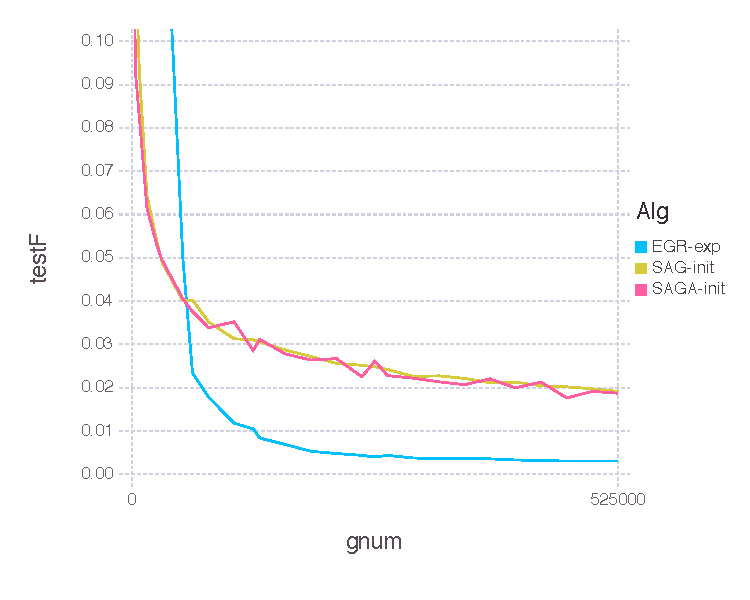
\includegraphics[width=\textwidth]{Figures/myrandBLtrueFfFinal-g.pdf}
           \caption{myrand}
       \end{subfigure}
       ~ %add desired spacing between images, e. g. ~, \quad, \qquad, \hfill etc.
         %(or a blank line to force the subfigure onto a new line)
         \begin{subfigure}[b]{0.45\textwidth}
           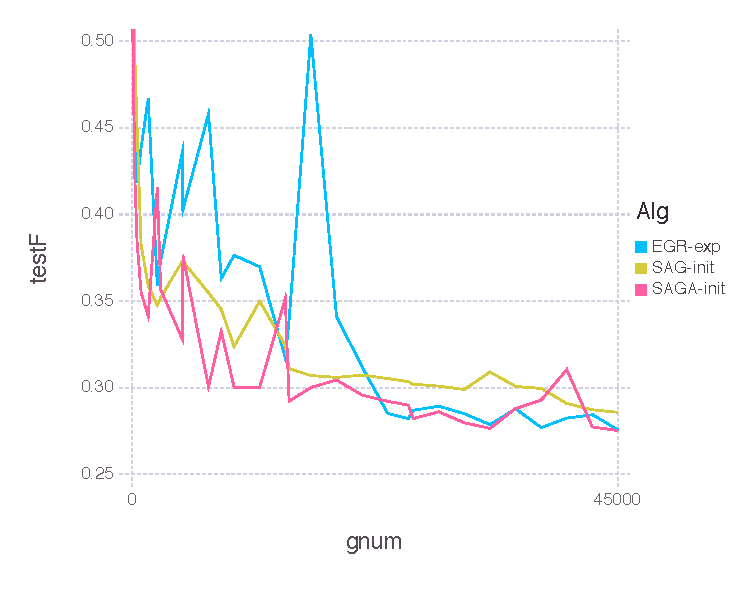
\includegraphics[width=\textwidth]{Figures/MNISTBLtrueFfFinal-g.pdf}
             \caption{MNIST}
         \end{subfigure}
       \caption{EGR vs other methods}\label{fig:myrandom}
   \end{figure}
   
   \begin{figure}[H]
       \centering
       \begin{subfigure}[b]{0.45\textwidth}
           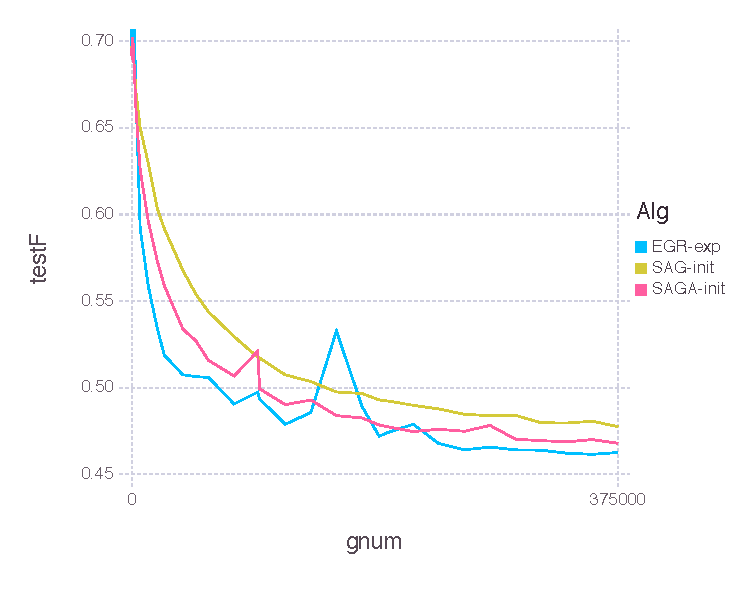
\includegraphics[width=\textwidth]{Figures/alphaGoodBLtrueFfFinal-g.pdf}
           \caption{alphaGood}
       \end{subfigure}
       ~ %add desired spacing between images, e. g. ~, \quad, \qquad, \hfill etc.
         %(or a blank line to force the subfigure onto a new line)
         \begin{subfigure}[b]{0.45\textwidth}
           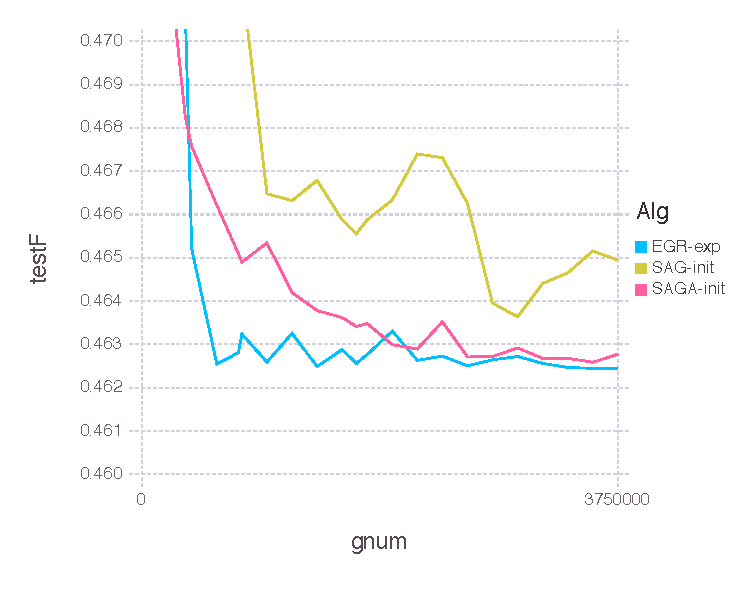
\includegraphics[width=\textwidth]{Figures/SUSYBLtrueFfFinal-g.pdf}
             \caption{SUSY}
         \end{subfigure}
       \caption{EGR vs other methods}\label{fig:alphaGoodom}
   \end{figure}
   
   
   \subsubsection{EGR Benchmarking}
   
   The three different growth rates (linear, quadratic, exponential) combined with two possible computation formulas for $y_k$ give rise to six methods, where each growth has an unspecified parameter. We tune it experimentally for each problem, and make observations of the effect of varying $r$ in each case. Finally, we make suggestions on good practical choices or $r$. 
   
   In all plots in this section, the vertical axis is the test function value, which serves as an approximation to $F$. We demonstrate the continuous progression of the algorithms toward the minimizer of $F$. The horizontal axis is the total number of sample gradients evaluated so far. This is an approximate measure of the total work the algorithm has performed, and is more informative than the more commonly used plots where the horizontal axis is the iteration counter. All experiements were stopped when the number of sample gradients evaluated reached the size of the complete training set. Note that for our choices of the growth rates, when $s_k=u_k$, this means that roughly half of the avaiable training points was seen by the algorithm. 
  The last remaining parameter, $\alpha$, was chosen to give the best testing function value at the end of the training epoch. A complete collection of these experiments for each of the six methods, on all four test problems can be seen in Figures \ref{fig:MNIST}, \ref{fig:alphaGood}, \ref{fig:myrand}, and \ref{fig:SUSY}. These extensive experiments are summarized in Figures \ref{fig:MNISTsummary}, \ref{fig:alphaGoodsummary}, \ref{fig:myrandsummary}, and \ref{fig:SUSYsummary} respectively. These summary plots show the best performing growth rates compared against each other. 

   

      \begin{figure}[H]
          \centering
          \begin{subfigure}[b]{0.45\textwidth}
              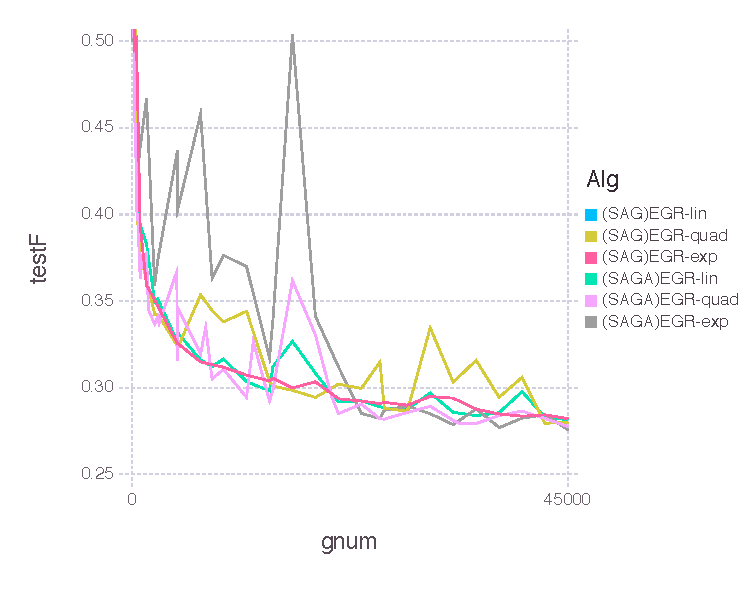
\includegraphics[width=\textwidth]{Figures/MNISTBLtrueFfFinal-1.pdf}
              \caption{MNIST}
          \end{subfigure}
          ~ %add desired spacing between images, e. g. ~, \quad, \qquad, \hfill etc. 
            %(or a blank line to force the subfigure onto a new line)
            \begin{subfigure}[b]{0.45\textwidth}
           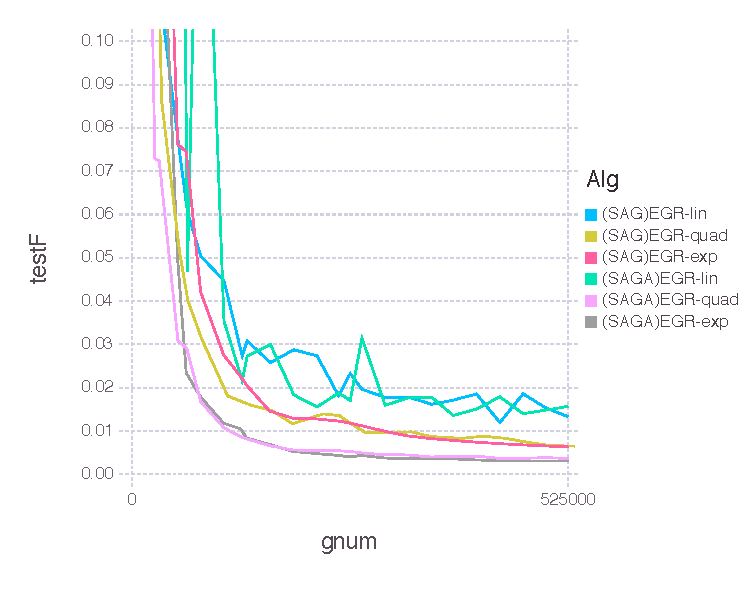
\includegraphics[width=\textwidth]{Figures/myrandBLtrueFfFinal-1.pdf}
                \caption{myrand}
            \end{subfigure}
          \caption{summary: all EGR methods}\label{fig:MNISTsummary}
      \end{figure}
   
   \begin{figure}[H]
       \centering
       \begin{subfigure}[b]{0.45\textwidth}
           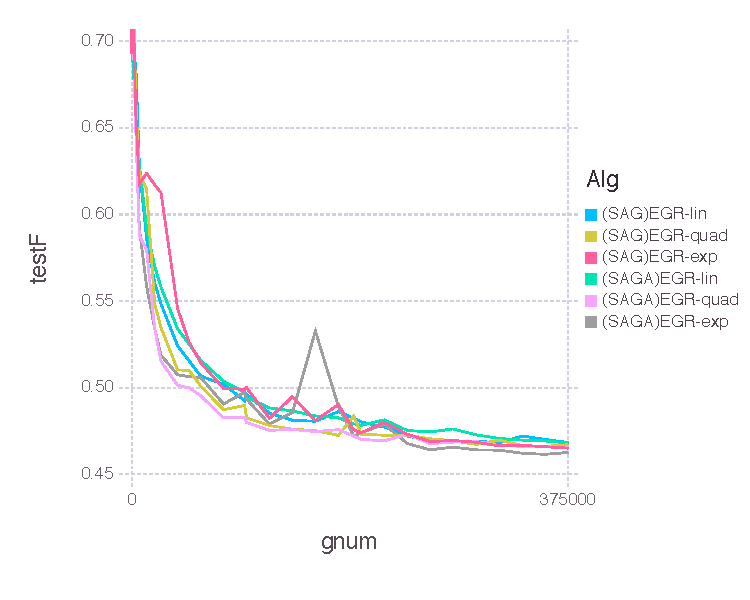
\includegraphics[width=\textwidth]{Figures/alphaGoodBLtrueFfFinal-1.pdf}
           \caption{alphaGood}
       \end{subfigure}
       ~ %add desired spacing between images, e. g. ~, \quad, \qquad, \hfill etc.
         %(or a blank line to force the subfigure onto a new line)
         \begin{subfigure}[b]{0.45\textwidth}
           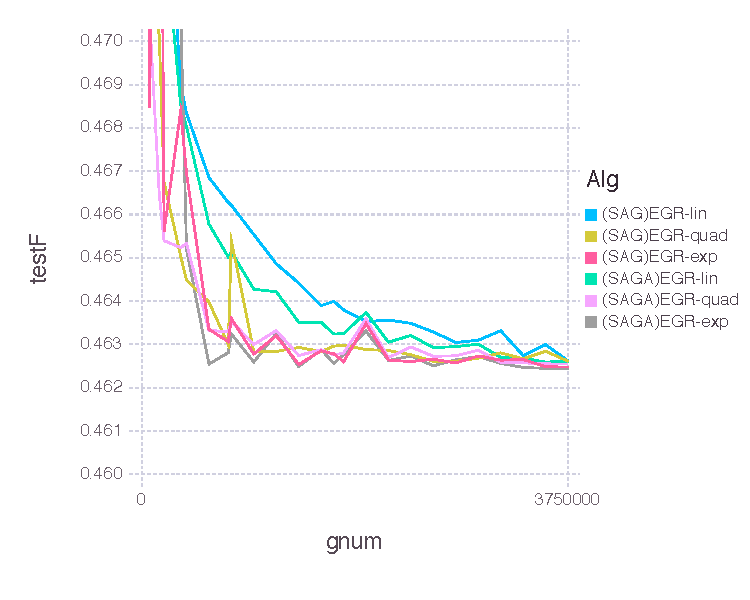
\includegraphics[width=\textwidth]{Figures/SUSYBLtrueFfFinal-1.pdf}
             \caption{SUSY}
         \end{subfigure}
       \caption{summary: all EGR methods}\label{fig:alphaGoodsummary}
   \end{figure}
   
   
		 
	     On problem MNIST, in Figure \ref{fig:MNIST}, we see that for EGR-lin(SAG) smaller batch sizes are preferable. When $r=1$, the method performs extremely well, but slightly increasing the batch to $r=10$ allows for significantly larger stepsizes to be taken. This closely follows the common knowledge about the need for mini-batching in SG methods. As $r$ increases, larger steplengths are needed for good performance: this is logical since the methods use more new information at each iteration, thus having less variance in the step directions. Large batch sizes do not work well, since the method is only able to take a few iterations in the allotted sample gradient evaluation limit. The EGR-lin(SAGA) version shows similar patterns, but a higher variance in the algorithm progression is seen. This is due to the fact that the SAG version of the algorithm places a much larger emphasis on the relatively stable term involving the summation of historic sample gradient information (which also implies that smaller stepsizes than in EGR-lin are needed). In the quadratic EGR-SAG growth rate case, the smallest $r$ tested gives the same method as the linear $r=1$ method because of rounding. The second growth rate (corresponding to $r=0.0001$) behaves identical to the smallest one initially, but approximately after the first half of the graph, the two plots diverge. This is because with the second growth rate the batch sizes start increasing from $s_k=u_k=1$. In the quadratic EGR-SAGA case, this sudden increase of the sample sizes enables the superior performance of the method. For the exponentially growing case, the same idea as before applies: A slightly increasing batch size in the latter iterations seems to benefit the stability and sometimes the performance of the methods.
   
	     In Figure~\ref{fig:MNISTsummary}, we combine these methods in two plots. The one on the left always shows the true progression of the algorithm to the minimizer, i.e. the current estimate of the function value of $F$. The plot on the right shows the same data plotted to display the current best solution. The EGR-SAGA methods with growing batch sizes at the end seem to work best in practice. We attribute this to the unbiased nature of the methods. We see that the best performing methods are the ones which increase the sample sizes at the end, instead of leaving them at a constant level. 
   
	     With the myrand dataset, the picture is slightly different. In Figure~\ref{fig:myrand}, we can see that the required growth rates are higher than for MNIST. In Figure~\ref{fig:myrandsummary}, we again see the clear advantage of using growing batch sizes, and of SAGA step computation formula over the SAG one. 
   
	     On the alphaGood dataset, and the SUSY dataset, the conclusions are similar. In Figure~\ref{fig:ss} we provide a plot of current sample size, $s_k+u_k$, at each iteration of the algorithm, on the MNIST dataset. The best performing growth rate choice seems to be the one where approximately for this first half of the algorithm progression the sample sizes are as small as possible, and only then start growing.
  
 
  \begin{figure}[H]
      \centering
      \begin{subfigure}[b]{0.45\textwidth}
          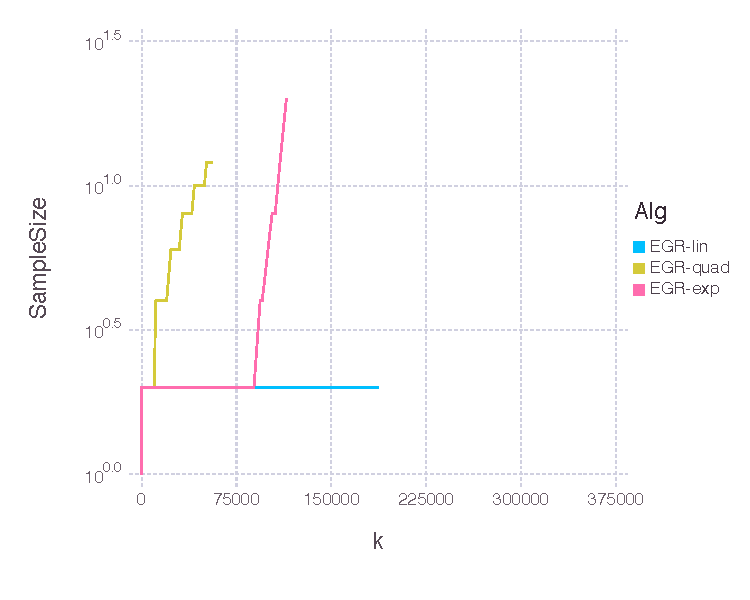
\includegraphics[width=\textwidth]{Figures/alphaGoodBLtrueSampleSizefFinal.pdf}
          \caption{alphaGood}
      \end{subfigure}
      ~ 
        \begin{subfigure}[b]{0.45\textwidth}
          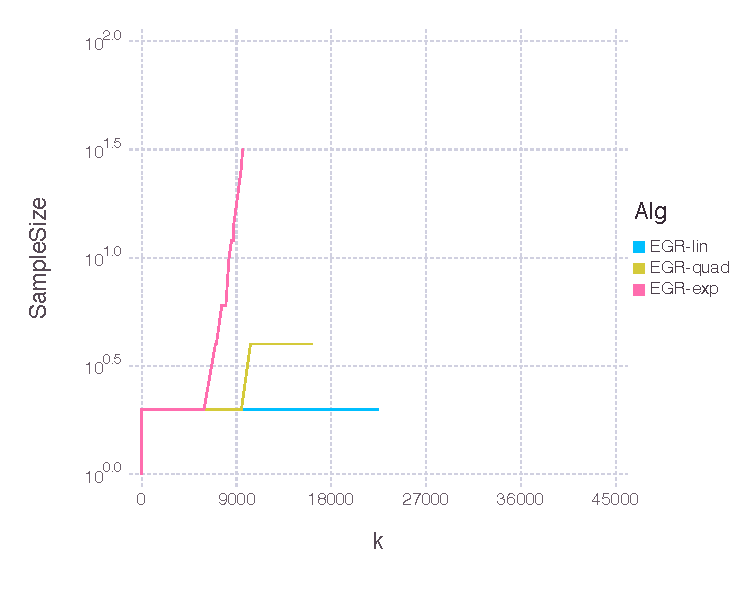
\includegraphics[width=\textwidth]{Figures/MNISTBLtrueSampleSizefFinal.pdf}
            \caption{MNIST}
        \end{subfigure}
      \caption{growth rates}\label{fig:alphaGoodsummary}
  \end{figure}
  
  
  \begin{figure}[H]
      \centering
      \begin{subfigure}[b]{0.45\textwidth}
          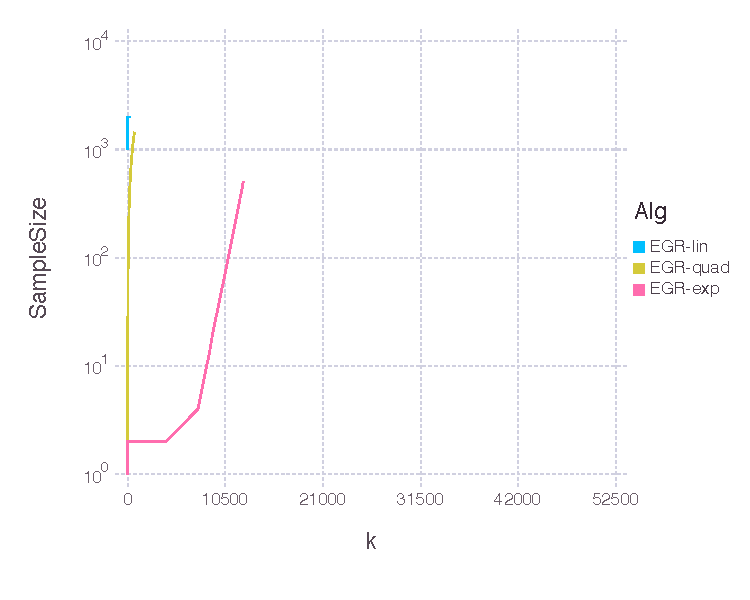
\includegraphics[width=\textwidth]{Figures/myrandBLtrueSampleSizefFinal.pdf}
          \caption{myrand}
      \end{subfigure}
      ~ %add desired spacing between images, e. g. ~, \quad, \qquad, \hfill etc.
        %(or a blank line to force the subfigure onto a new line)
        \begin{subfigure}[b]{0.45\textwidth}
          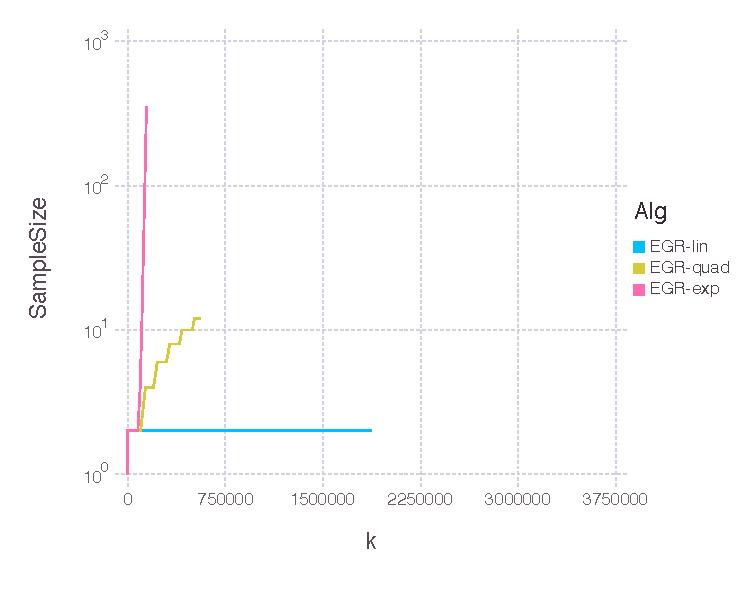
\includegraphics[width=\textwidth]{Figures/SUSYBLtrueSampleSizefFinal.pdf}
            \caption{SUSY}
        \end{subfigure}
      \caption{growth rates}\label{fig:alphaGoodsummary}
  \end{figure}
  

  
  
  
  
  
  
   \subsubsection{Only Add Comparison}

   
   The only-add option in EGR includes many existing methods, such as SG and DSS. We empirically compare the performance of our new methods with SG and DSS. The Stochastic Gradient method enjoys immense popularity in both the optimization and the machine learning communities, and when carefully tuned can outperform any known modern method. The tuning often involves intricate step size strategies. We do not attempt to compare with the best SG implementation, rather we demonstrate the benefits of using the EGR scheme, compared to SG, with both methods using a constant step size. The DSS method tested uses a sample size identical to the one suggested by EGR, to make the per-iteration comparison fair. The plots for each problem can be found in Figures \ref{fig:MNISToa},  \ref{fig:myrandoa},  \ref{fig:alphaGoodoa},  \ref{fig:SUSYoa}.
   

   \begin{figure}[H]
       \centering
       \begin{subfigure}[b]{0.45\textwidth}
           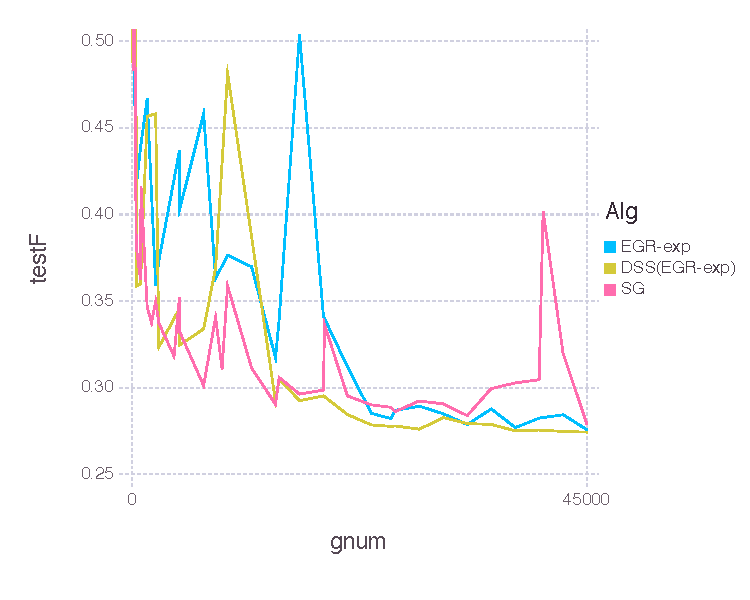
\includegraphics[width=\textwidth]{Figures/MNISTBLtrueFfFinal-dss.pdf}
           \caption{MNIST}
       \end{subfigure}
       ~ %add desired spacing between images, e. g. ~, \quad, \qquad, \hfill etc.
         %(or a blank line to force the subfigure onto a new line)
         \begin{subfigure}[b]{0.45\textwidth}
           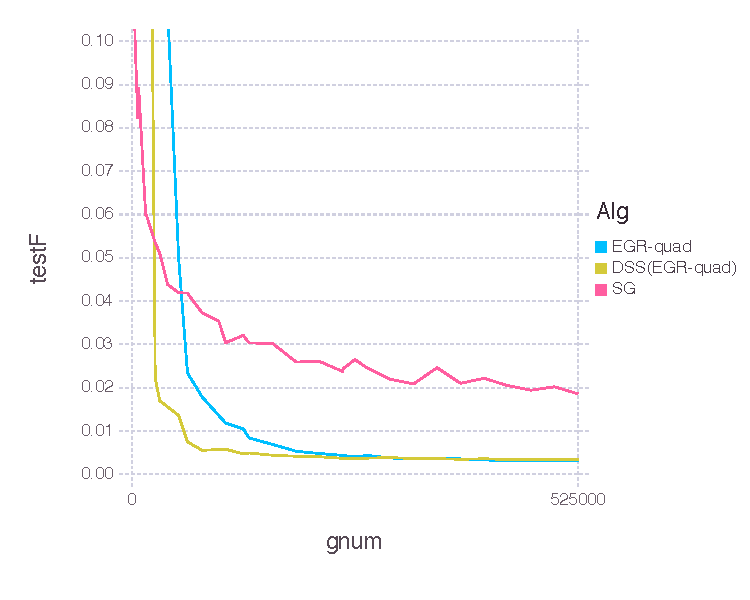
\includegraphics[width=\textwidth]{Figures/myrandBLtrueFfFinal-dss.pdf}
             \caption{myrand}
         \end{subfigure}
       \caption{EGR vs only-add methods}\label{fig:MNISToa}
   \end{figure}
   
   \begin{figure}[H]
       \centering
       \begin{subfigure}[b]{0.45\textwidth}
           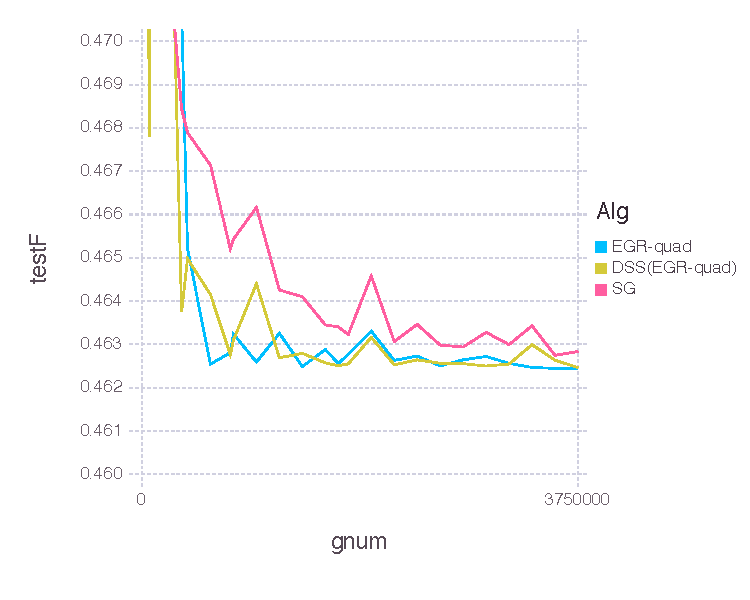
\includegraphics[width=\textwidth]{Figures/SUSYBLtrueFfFinal-dss.pdf}
           \caption{SUSY}
       \end{subfigure}
       ~ %add desired spacing between images, e. g. ~, \quad, \qquad, \hfill etc.
         %(or a blank line to force the subfigure onto a new line)
         \begin{subfigure}[b]{0.45\textwidth}
           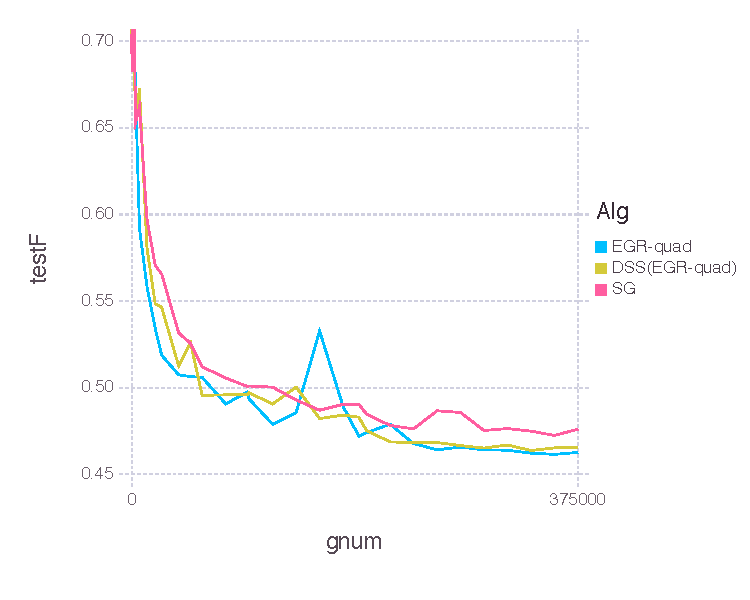
\includegraphics[width=\textwidth]{Figures/alphaGoodBLtrueFfFinal-dss.pdf}
             \caption{alphaGood}
         \end{subfigure}
       \caption{EGR vs only-add methods}\label{fig:SUSYoa}
   \end{figure}
   
   These plots show that the benefit of having multiple sample gradients evaluated at some iterations is advantageous to having a single one being evaluated at each step. In most of our experiments, DSS performed slightly better, because it was able to see all data while EGR only half. This advantage is not uniform, and we cannot make a justifiable recommendation of using one over the other.
   
   \subsubsection{Memory Reduction Techniques in Practice}
   
   The following experiments show the algorithm progress after 40 passes over the data. Only two types of chunking are tested: SAG and SAGA chunking. The labels are in the format \texttt{algorithm numChunks StepsizePower}. The stepsizes were tuned to give the best final function value. 
   
   The follwing experiements show comparisons of the aggregated gradient methods SAG and SAGA with respect to Batching vs Chunking. We conducted experiments comparing Chunking vs Batching on three datasets, and two aggregated gradient methods: SAG and SAGA. This experiment was suggested to verify the previous chunking results (on pages 41-43), because these previous experiments suggested that the chunking idea is not working well in practice. 

   The new experiments are ran with 40 equivalent passes over the data, and stepsizes were chosen to give the best possible function value over the progress of all iterations. Each method was tested with the following two configurations:
   a) Batching - batches of size 2, chunks of size 1  (blue and red on plots)
   b) Chunking - chunks of size 2, batches of size 1 (yellow and green on plots)

   The chunking methods seem to perform much worse than the equivalent batching methods.

\section{Final Remarks} \label{finalr}


 \small 
\bibliographystyle{plain}

\bibliography{../References/references}

\appendix 

\section{EGR Growth Rates Detailed} \label{appendix:EGRGrowthRatesDetailed}
   
   \begin{figure}[H]
       \centering
\begin{subfigure}[b]{0.45\textwidth}
           \includegraphics[width=\textwidth]{Figures/MNISTBLtrueffFinal-linfalse.pdf}
           \caption{EGR-lin(SAG)}
       \end{subfigure}
       ~ %add desired spacing between images, e. g. ~, \quad, \qquad, \hfill etc. 
         %(or a blank line to force the subfigure onto a new line)
       \begin{subfigure}[b]{0.45\textwidth}
           \includegraphics[width=\textwidth]{Figures/MNISTBLtrueffFinal-lintrue.pdf}
           \caption{EGR-lin(SAGA)} 
       \end{subfigure}
	   
	    \begin{subfigure}[b]{0.45\textwidth}
           \includegraphics[width=\textwidth]{Figures/MNISTBLtrueffFinal-quadfalse.pdf}
           \caption{EGR-quad(SAG)}
       \end{subfigure}
       ~ %add desired spacing between images, e. g. ~, \quad, \qquad, \hfill etc. 
         %(or a blank line to force the subfigure onto a new line)
       \begin{subfigure}[b]{0.45\textwidth}
           \includegraphics[width=\textwidth]{Figures/MNISTBLtrueffFinal-quadtrue.pdf}
           \caption{EGR-quad(SAGA)}
       \end{subfigure}
	   
       \begin{subfigure}[b]{0.45\textwidth}
           \includegraphics[width=\textwidth]{Figures/MNISTBLtrueffFinal-expfalse.pdf}
           \caption{EGR-exp(SAG)}
       \end{subfigure}
       ~ %add desired spacing between images, e. g. ~, \quad, \qquad, \hfill etc. 
         %(or a blank line to force the subfigure onto a new line)
         \begin{subfigure}[b]{0.45\textwidth}
             \includegraphics[width=\textwidth]{Figures/MNISTBLtrueffFinal-exptrue.pdf}
             \caption{EGR-exp(SAGA)}
         \end{subfigure}
       \caption{MNIST detailed: Comparing various growth rates. In the legend, $r$ is the parameter from Table \ref{tab1} and $a=log_2(\alpha)$ where $\alpha$ is the constant stepsize parameter.}\label{fig:MNIST}
   \end{figure}
   
      \begin{figure}[H]
          \centering
   \begin{subfigure}[b]{0.45\textwidth}
              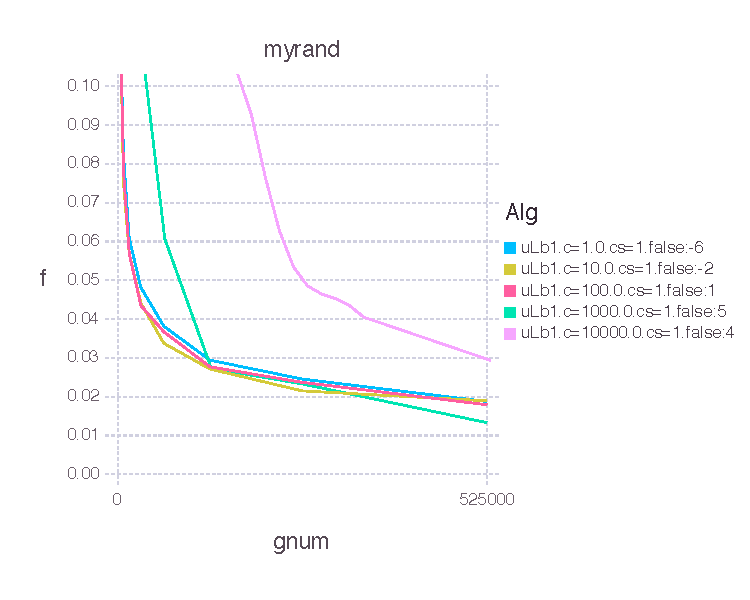
\includegraphics[width=\textwidth]{Figures/myrandBLtrueffFinal-linfalse.pdf}
              \caption{EGR-lin(SAG)}
          \end{subfigure}
          ~ %add desired spacing between images, e. g. ~, \quad, \qquad, \hfill etc. 
            %(or a blank line to force the subfigure onto a new line)
          \begin{subfigure}[b]{0.45\textwidth}
              \includegraphics[width=\textwidth]{Figures/myrandBLtrueffFinal-lintrue.pdf}
              \caption{EGR-lin(SAGA)} 
          \end{subfigure}
	   
   	    \begin{subfigure}[b]{0.45\textwidth}
              \includegraphics[width=\textwidth]{Figures/myrandBLtrueffFinal-quadfalse.pdf}
              \caption{EGR-quad(SAG)}
          \end{subfigure}
          ~ %add desired spacing between images, e. g. ~, \quad, \qquad, \hfill etc. 
            %(or a blank line to force the subfigure onto a new line)
          \begin{subfigure}[b]{0.45\textwidth}
              \includegraphics[width=\textwidth]{Figures/myrandBLtrueffFinal-quadtrue.pdf}
              \caption{EGR-quad(SAGA)}
          \end{subfigure}
	   
          \begin{subfigure}[b]{0.45\textwidth}
              \includegraphics[width=\textwidth]{Figures/myrandBLtrueffFinal-expfalse.pdf}
              \caption{EGR-exp(SAG)}
          \end{subfigure}
          ~ %add desired spacing between images, e. g. ~, \quad, \qquad, \hfill etc. 
            %(or a blank line to force the subfigure onto a new line)
            \begin{subfigure}[b]{0.45\textwidth}
                \includegraphics[width=\textwidth]{Figures/myrandBLtrueffFinal-exptrue.pdf}
                \caption{EGR-exp(SAGA)}
            \end{subfigure}
          \caption{myrand detailed: Comparing various growth rates. In the legend, $r$ is the parameter from Table \ref{tab1} and $a=log_2(\alpha)$ where $\alpha$ is the constant stepsize parameter.}\label{fig:myrand}
      \end{figure}
   
      \begin{figure}[H]
          \centering
   \begin{subfigure}[b]{0.45\textwidth}
              \includegraphics[width=\textwidth]{Figures/alphaGoodBLtrueffFinal-linfalse.pdf}
              \caption{EGR-lin(SAG)}
          \end{subfigure}
          ~ %add desired spacing between images, e. g. ~, \quad, \qquad, \hfill etc. 
            %(or a blank line to force the subfigure onto a new line)
          \begin{subfigure}[b]{0.45\textwidth}
              \includegraphics[width=\textwidth]{Figures/alphaGoodBLtrueffFinal-lintrue.pdf}
              \caption{EGR-lin(SAGA)} 
          \end{subfigure}
	   
   	    \begin{subfigure}[b]{0.45\textwidth}
              \includegraphics[width=\textwidth]{Figures/alphaGoodBLtrueffFinal-quadfalse.pdf}
              \caption{EGR-quad(SAG)}
          \end{subfigure}
          ~ %add desired spacing between images, e. g. ~, \quad, \qquad, \hfill etc. 
            %(or a blank line to force the subfigure onto a new line)
          \begin{subfigure}[b]{0.45\textwidth}
              \includegraphics[width=\textwidth]{Figures/alphaGoodBLtrueffFinal-quadtrue.pdf}
              \caption{EGR-quad(SAGA)}
          \end{subfigure}
	   
          \begin{subfigure}[b]{0.45\textwidth}
              \includegraphics[width=\textwidth]{Figures/alphaGoodBLtrueffFinal-expfalse.pdf}
              \caption{EGR-exp(SAG)}
          \end{subfigure}
          ~ %add desired spacing between images, e. g. ~, \quad, \qquad, \hfill etc. 
            %(or a blank line to force the subfigure onto a new line)
            \begin{subfigure}[b]{0.45\textwidth}
                \includegraphics[width=\textwidth]{Figures/alphaGoodBLtrueffFinal-exptrue.pdf}
                \caption{EGR-exp(SAGA)}
            \end{subfigure}
          \caption{alphaGood detailed: Comparing various growth rates. In the legend, $r$ is the parameter from Table \ref{tab1} and $a=log_2(\alpha)$ where $\alpha$ is the constant stepsize parameter.}\label{fig:alphaGood}
      \end{figure}
   
      \begin{figure}[H]
          \centering
   \begin{subfigure}[b]{0.45\textwidth}
              \includegraphics[width=\textwidth]{Figures/SUSYBLtrueffFinal-linfalse.pdf}
              \caption{EGR-lin(SAG)}
          \end{subfigure}
          ~ %add desired spacing between images, e. g. ~, \quad, \qquad, \hfill etc. 
            %(or a blank line to force the subfigure onto a new line)
          \begin{subfigure}[b]{0.45\textwidth}
              \includegraphics[width=\textwidth]{Figures/SUSYBLtrueffFinal-lintrue.pdf}
              \caption{EGR-lin(SAGA)} 
          \end{subfigure}
	   
   	    \begin{subfigure}[b]{0.45\textwidth}
              \includegraphics[width=\textwidth]{Figures/SUSYBLtrueffFinal-quadfalse.pdf}
              \caption{EGR-quad(SAG)}
          \end{subfigure}
          ~ %add desired spacing between images, e. g. ~, \quad, \qquad, \hfill etc. 
            %(or a blank line to force the subfigure onto a new line)
          \begin{subfigure}[b]{0.45\textwidth}
              \includegraphics[width=\textwidth]{Figures/SUSYBLtrueffFinal-quadtrue.pdf}
              \caption{EGR-quad(SAGA)}
          \end{subfigure}
	   
          \begin{subfigure}[b]{0.45\textwidth}
              \includegraphics[width=\textwidth]{Figures/SUSYBLtrueffFinal-expfalse.pdf}
              \caption{EGR-exp(SAG)}
          \end{subfigure}
          ~ %add desired spacing between images, e. g. ~, \quad, \qquad, \hfill etc. 
            %(or a blank line to force the subfigure onto a new line)
            \begin{subfigure}[b]{0.45\textwidth}
                \includegraphics[width=\textwidth]{Figures/SUSYBLtrueffFinal-exptrue.pdf}
                \caption{EGR-exp(SAGA)}
            \end{subfigure}
          \caption{SUSY detailed: Comparing various growth rates. In the legend, $r$ is the parameter from Table \ref{tab1} and $a=log_2(\alpha)$ where $\alpha$ is the constant stepsize parameter.}\label{fig:SUSY}
      \end{figure}


\end{document}
